\documentclass{article}

\usepackage[T1]{fontenc}
\usepackage[utf8]{inputenc}
\usepackage[brazilian]{babel}
\usepackage{graphicx}
\usepackage[export]{adjustbox}[2011/08/13]
\usepackage{float}
\usepackage[pdftex]{hyperref}
\usepackage{epstopdf}
\usepackage{etoolbox}
\usepackage{amsmath}
\usepackage{amsfonts}
\usepackage{amssymb}
\usepackage{caption}
\usepackage{subcaption}
\usepackage{setspace}
\usepackage{tikz}
\usepackage{listings}
\usepackage{xcolor} 

\bibliographystyle{eric}
\patchcmd{\thebibliography}{\section*}{\section}{}{}


\newcommand{\R}{\ensuremath{\mathbb{R}}}
\newcommand{\Prob}{\ensuremath{\mathbb{P}}}
\newcommand{\K}{\ensuremath{\mathbb{K}}}
\newcommand{\U}{\ensuremath{\mathbb{U}}}
\newcommand{\N}{\ensuremath{\mathbb{N}}}
\newcommand{\Lg}{\ensuremath{\mathbb{L}}}
\newcommand{\T}{\ensuremath{\rm Tr}}
\newcommand{\sg}{{\sigma(x_k)}}

\newcommand{\G}{\ensuremath{\mathcal{G}}}
\newcommand{\F}{\ensuremath{\mathcal{F}}}
\newcommand{\C}{\ensuremath{\mathcal{C}}}
\newcommand{\E}{\ensuremath{\mathcal{E}}}
\newcommand{\Hn}{\ensuremath{\mathcal{H}}}
\newcommand{\Hoo}{\ensuremath{\mathcal{H}_\infty}}
\newcommand{\Hop}{\ensuremath{\mathcal{H}_{op}}}
% --------------------------------------------------
\newtheorem{theo}{Teorema}
\newtheorem{exa}{Exemplo}
\newtheorem{lemm}{Lema}
\newtheorem{coro}{Corolário}
\newtheorem{defn}{Definição}[section]

\begin{document}

\begin{titlepage}
\begin{center}

\newcommand{\HRule}{\rule{\linewidth}{0.5mm}}
% Upper part of the page. The '~' is needed because \\
% only works if a paragraph has started.

\includegraphics[width=0.15\textwidth]{logoUnicamp}~\\[1cm]

\textsc{\LARGE Universidade Estadual de Campinas}\\[1.5cm]

\textsc{\Large Faculdade de Engenharia Mecânica}\\[0.5cm]

% Title
\HRule \\[0.4cm]
{ \huge \bfseries ES664 - Laboratório de Eletrônica para Automação Industrial\\ \vspace{1cm} Relatório - Experimento 4\\
\Large{Acionamento de motor DC} \\[0.4cm] }

\HRule \\[1.5cm]

% Author and supervisor
\begin{minipage}{0.6\textwidth}
\begin{flushleft} \large
\emph{Nome:}\\
Daniel Dello Russo Oliveira\\Marcelli Tiemi Kian
\end{flushleft}
\end{minipage}
\begin{minipage}{0.2\textwidth}
\begin{flushright} \large
\emph{RA}\\ 101918\\117892
\end{flushright}
\end{minipage}

\vfill

% Bottom of the page
{\large \today}

\end{center}
\end{titlepage}


\onehalfspacing
\section{Objetivos}
	Essa simulação tem como objetivo o estudo dos motores DC de ímãs permanentes e sua acionamento através de topologias baseadas em retificadores controlados.
	 
\section{Simualações}
\subsection{Modelagem de um motor DC: diagrama de blocos}
Através do Simulink implementamos a função de transferência de um motor DC através do diagrama de blocos apresentado na figura \ref{fig:sim1}.
\begin{figure}[H]
	\centering
	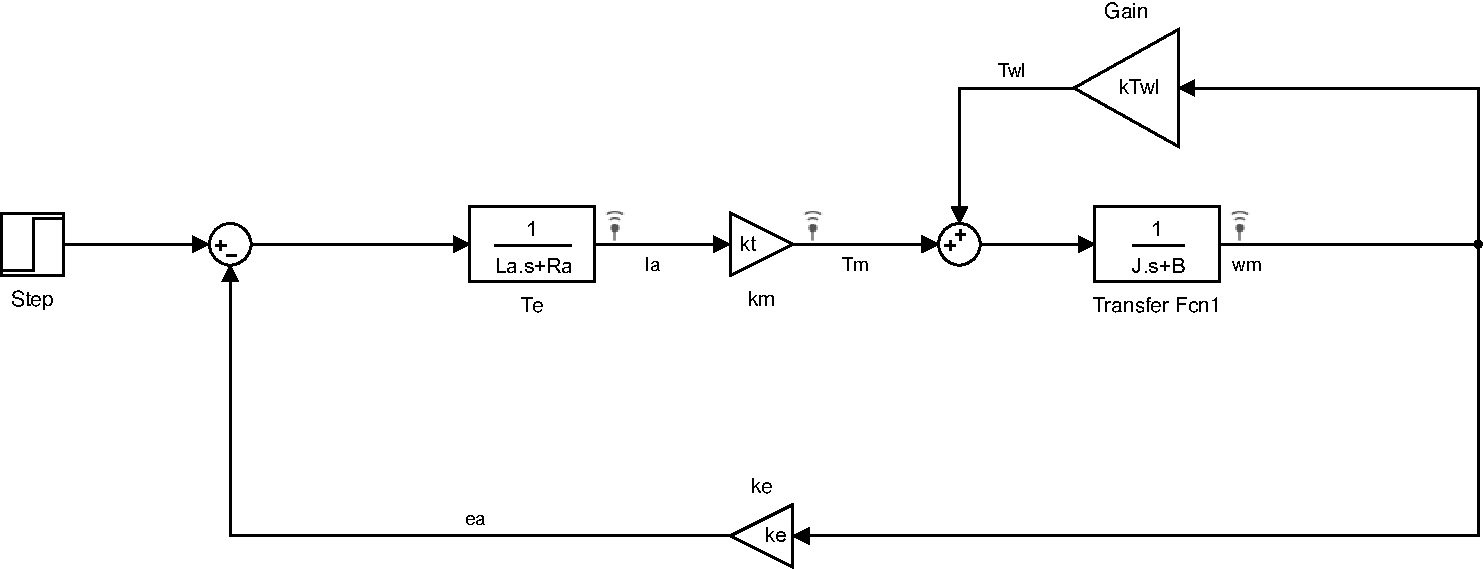
\includegraphics[width=\linewidth]{matlab/sim1}
	\caption{Motor DC implementado através do diagrama de blocos}
	\label{fig:sim1}
\end{figure}
Separamos a parte elétrica e mecânica da função de transferência do motor conforme pode ser visto na figura. Adotamos os valores apresentados no roteiro para os parâmetros do motor ($R_a = 1.6 \Omega$, $L_a = 667 \mu H$, $1.1 \times 10^{-4} kg\ m^2$, $B = 1.24 \times 10^{-4} J\ s/rad$, $k_e = 0.038 V\ s/rad$ e $k_t = 0.038 N\ m/A$).

Simulamos a resposta do motor sem carga a um degrau de 24V obtendo as curvas apresentadas na figura \ref{fig:res1}

\begin{figure}[H]
	\centering
	\begin{subfigure}[b]{0.49\linewidth}
		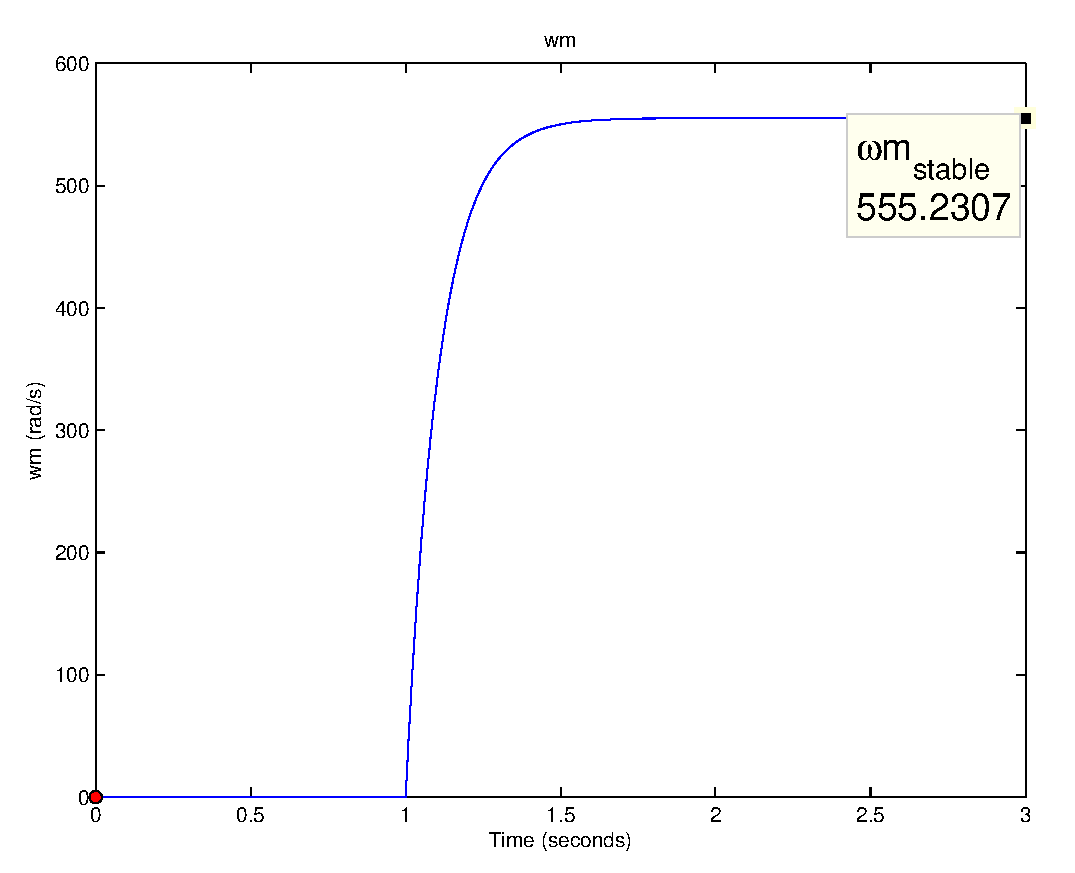
\includegraphics[width=\linewidth]{matlab/wm1}
		\caption{Velocidade Angular}
	\end{subfigure}
	\begin{subfigure}[b]{0.49\linewidth}
		\centering
		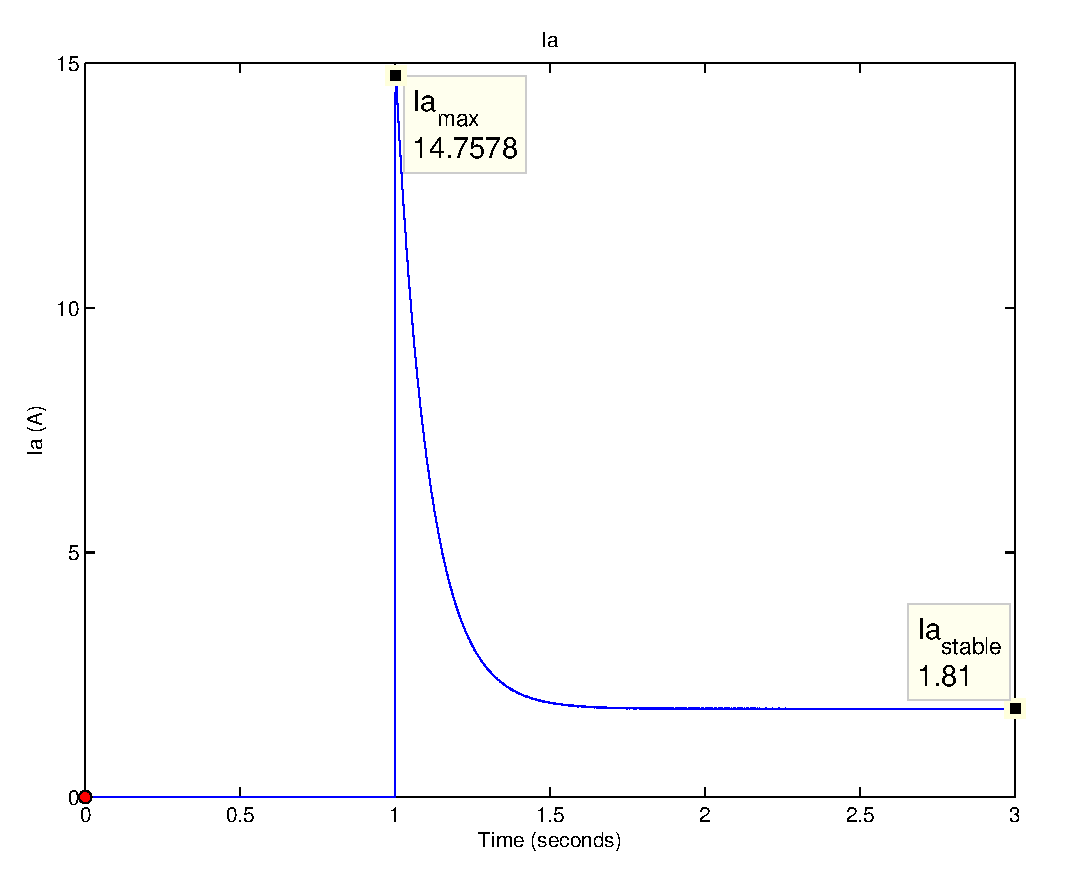
\includegraphics[width=\linewidth]{matlab/ia1}
		\caption{Corrente de armadura}
	\end{subfigure}
	\begin{subfigure}[b]{0.49\linewidth}
		\centering
		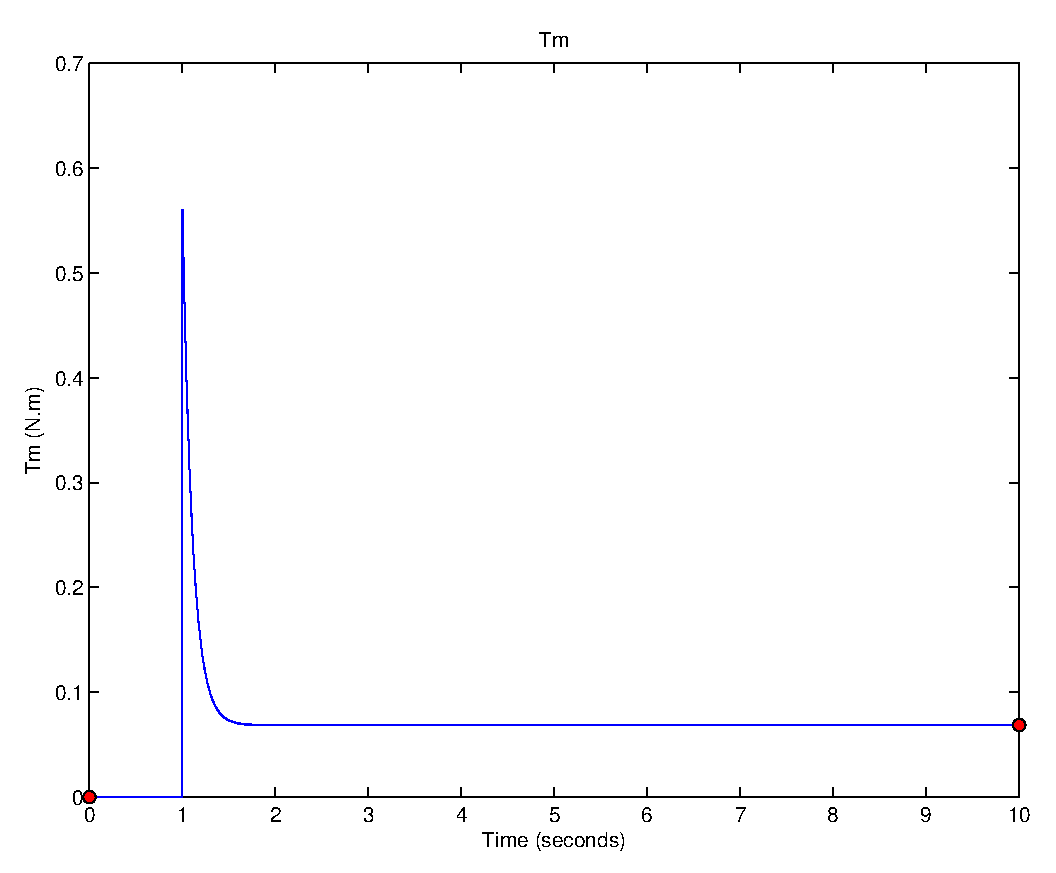
\includegraphics[width=\linewidth]{matlab/tm1}
		\caption{Torque do motor}
	\end{subfigure}
	\caption{Curvas de resposta do motor sem carga}
	\label{fig:res1}
\end{figure}

Colocamos então uma carga proporcional à velocidade no nosso motor (de função $Twl = - 5\times10^{-4}\omega_m$) e simulamos a resposta do motor ao mesmo degrau de entrada, obtendo as curvas da figura \ref{fig:res2}

\begin{figure}[H]
	\centering
	\begin{subfigure}[b]{0.49\linewidth}
		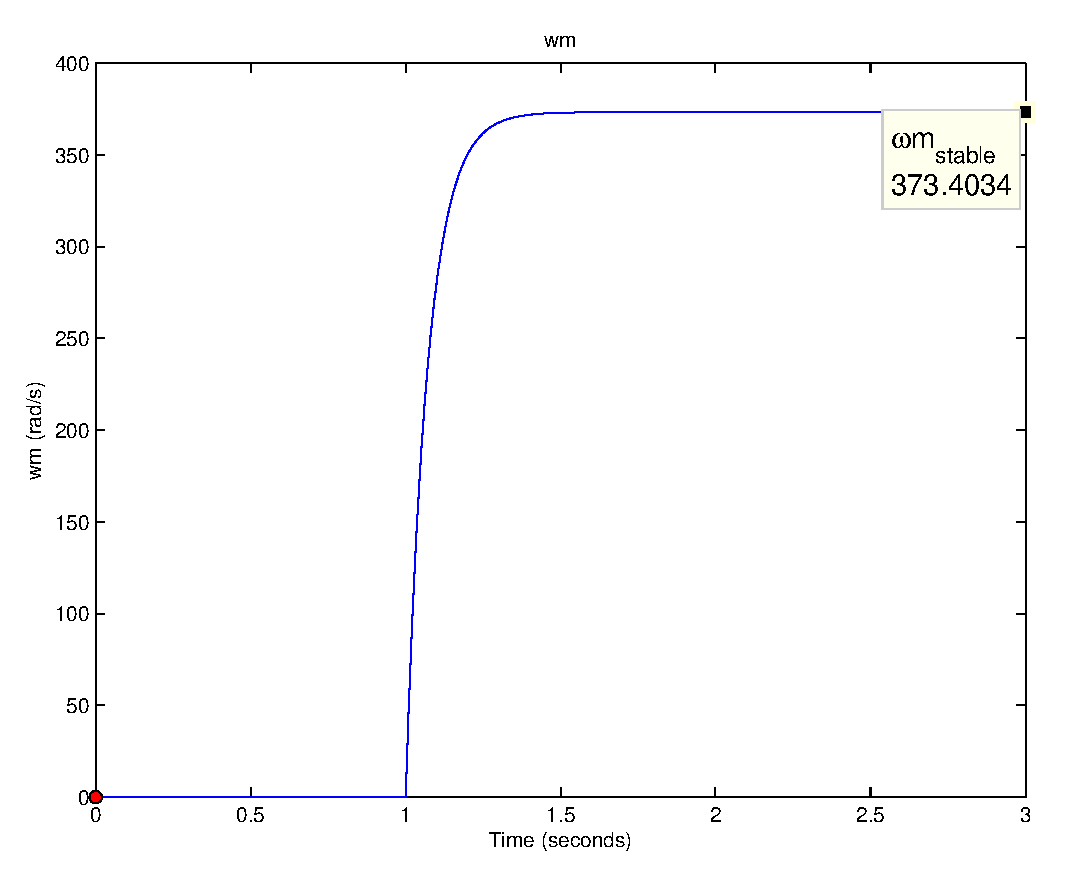
\includegraphics[width=\linewidth]{matlab/wm2}
		\caption{Velocidade Angular}
	\end{subfigure}
	\begin{subfigure}[b]{0.49\linewidth}
		\centering
		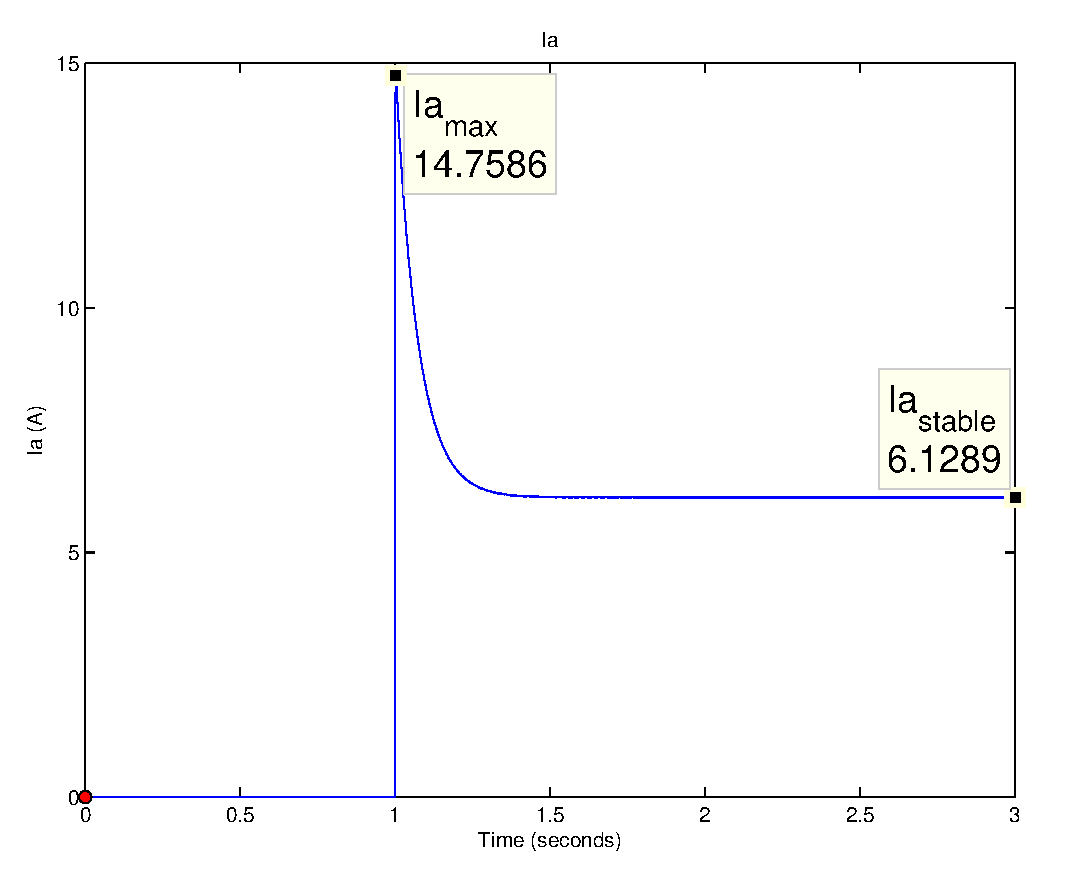
\includegraphics[width=\linewidth]{matlab/ia2}
		\caption{Corrente de armadura}
	\end{subfigure}
	\begin{subfigure}[b]{0.49\linewidth}
		\centering
		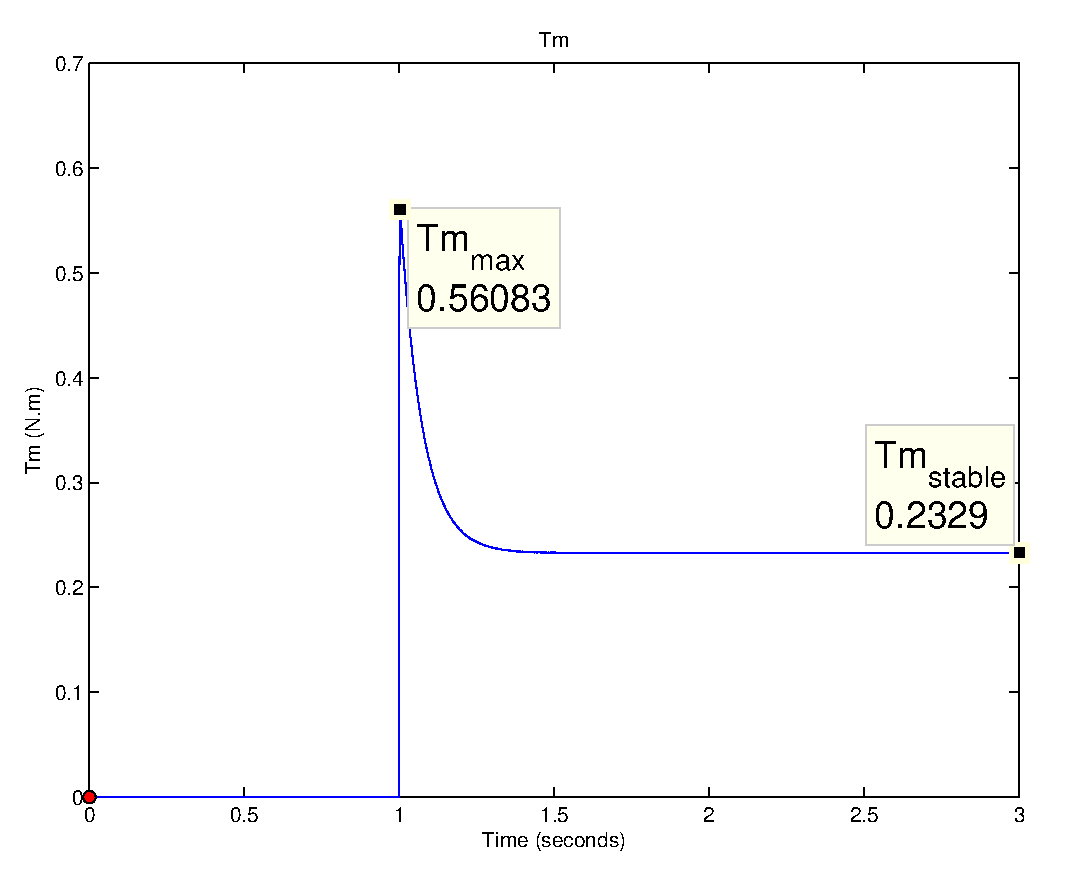
\includegraphics[width=\linewidth]{matlab/tm2}
		\caption{Torque do motor}
	\end{subfigure}
	\caption{Curvas de resposta do motor com carga proporcional à velocidade}
	\label{fig:res2}
\end{figure}

\subsection{Modelagem de um motor DC: SimPowerSystems}
Utilizando a biblioteca SimPowerSystems do Simulink implementamos o mesmo motor DC, agora utilizando o modelo disponível na biblioteca, conforme apresentado na figura \ref{fig:sim2}.
\begin{figure}[H]
	\centering
	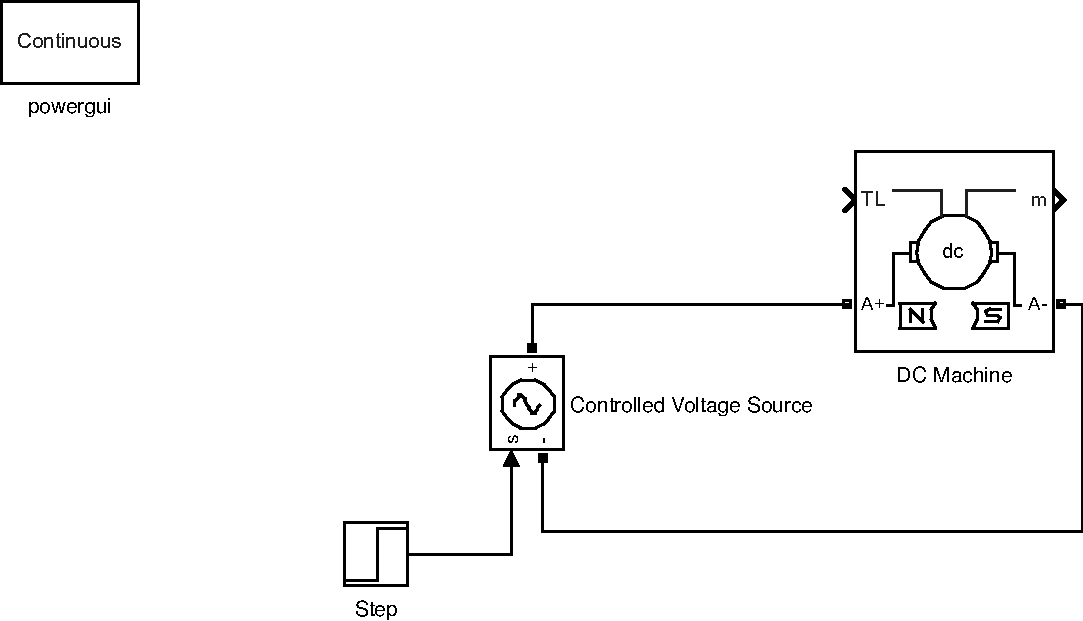
\includegraphics[width=0.6\linewidth]{matlab/sim2}
	\caption{Motor DC implementado através da biblioteca SimPowerSystems}
	\label{fig:sim2}
\end{figure}

Simulamos a resposta do motor sem carga a o mesmo degrau de 24V obtendo as curvas apresentadas na figura \ref{fig:res3}

\begin{figure}[H]
	\centering
	\begin{subfigure}[b]{0.49\linewidth}
		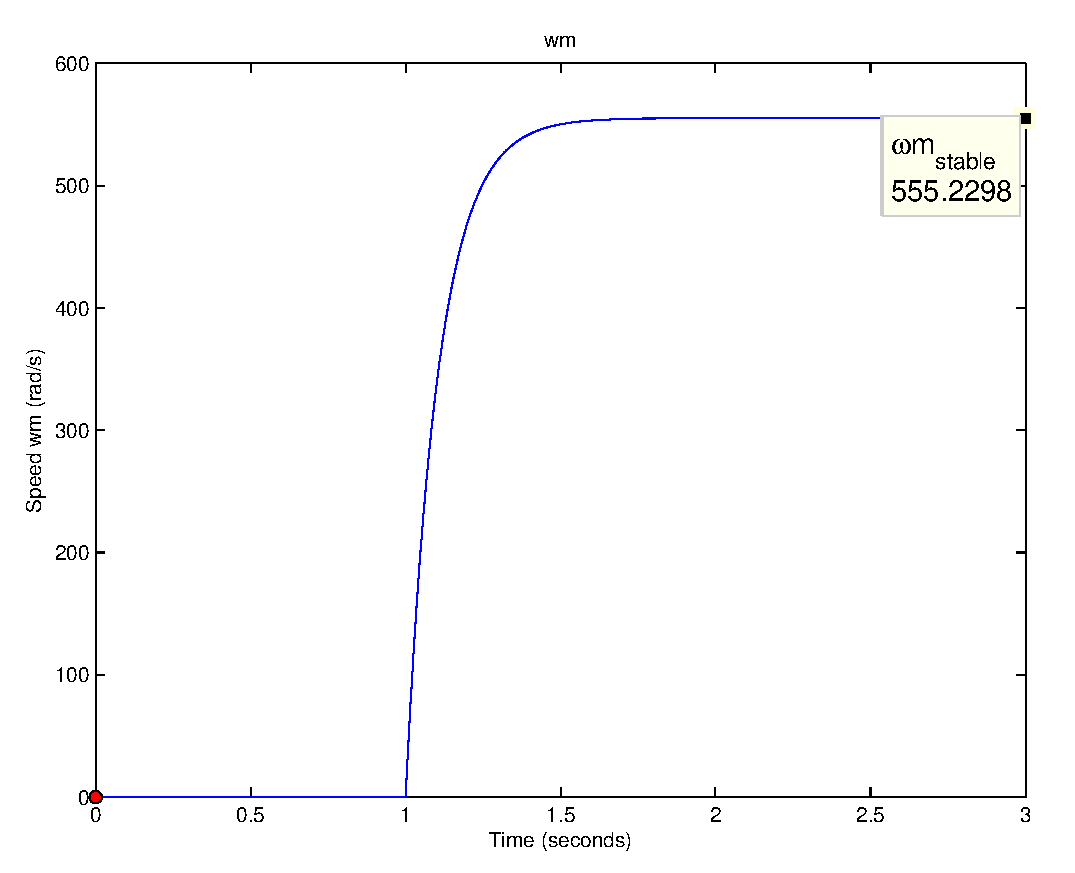
\includegraphics[width=\linewidth]{matlab/wm3}
		\caption{Velocidade Angular}
	\end{subfigure}
	\begin{subfigure}[b]{0.49\linewidth}
		\centering
		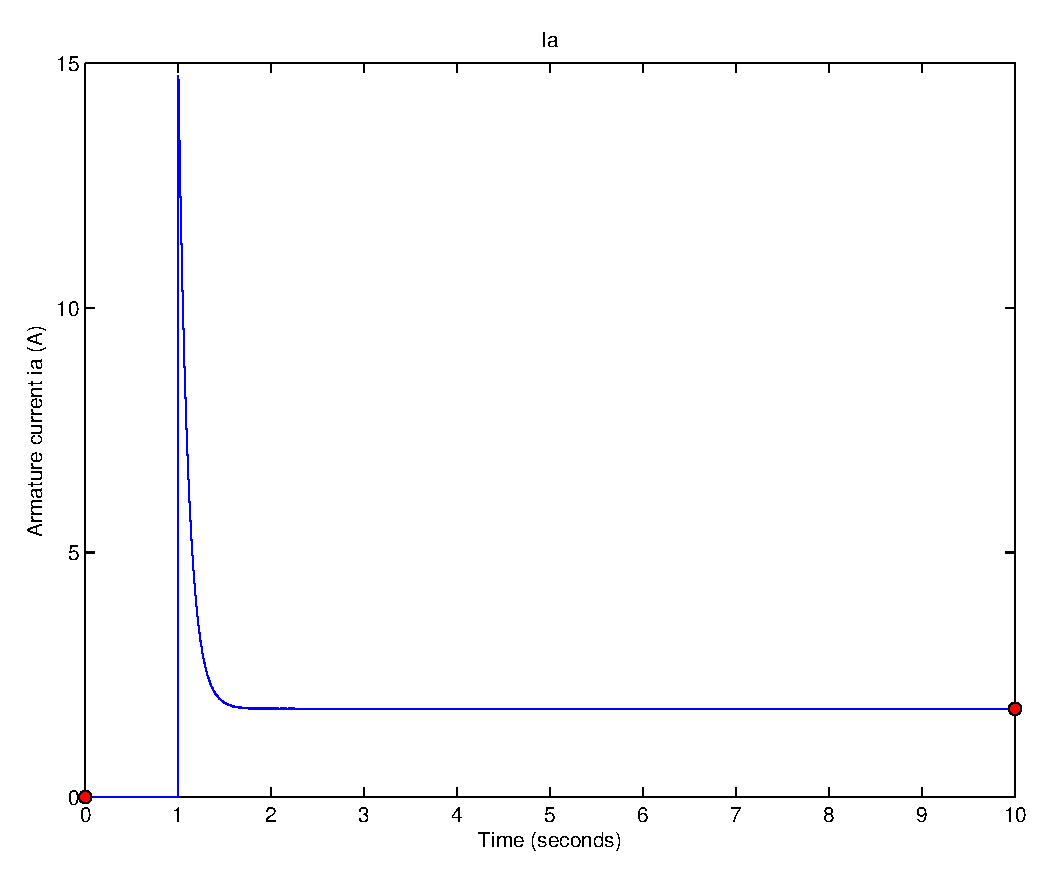
\includegraphics[width=\linewidth]{matlab/ia3}
		\caption{Corrente de armadura}
	\end{subfigure}
	\begin{subfigure}[b]{0.49\linewidth}
		\centering
		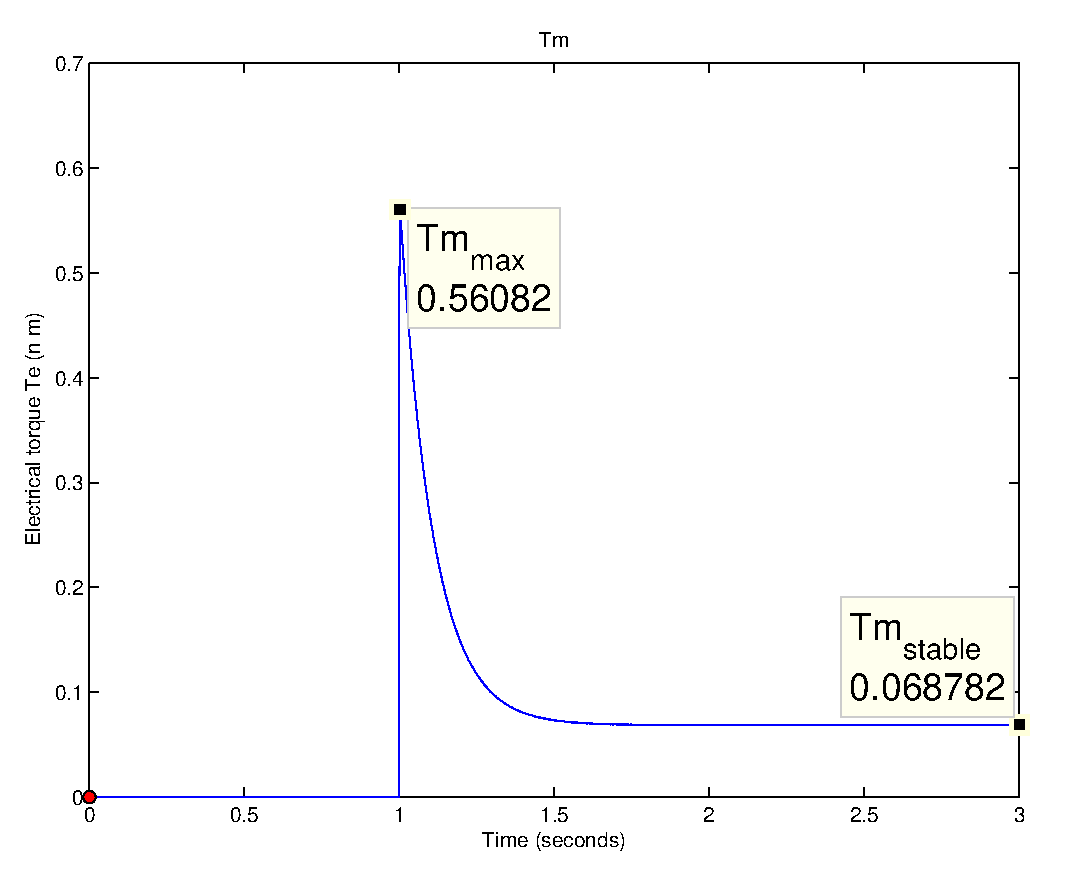
\includegraphics[width=\linewidth]{matlab/tm3}
		\caption{Torque do motor}
	\end{subfigure}
	\caption{Curvas de resposta do motor sem carga}
	\label{fig:res3}
\end{figure}

Como podemos ver os resultados são bastante semelhantes aos apresentados na figura \ref{fig:res1}, se não praticamente idênticos. Como podemos ver nosso modelo por blocos e o modelo utilizado internamente pela biblioteca são bastante semelhantes.

\subsection{ Acionamento de motor DC com retificador controlado}
Conectamos um retificador monofásico controlado de onda completa no nosso motor alimentado por uma fonte alternada (24 V rms@60 Hz), conforme pode ser visto na figura \ref{fig:sim3}.
\begin{figure}[H]
	\centering
	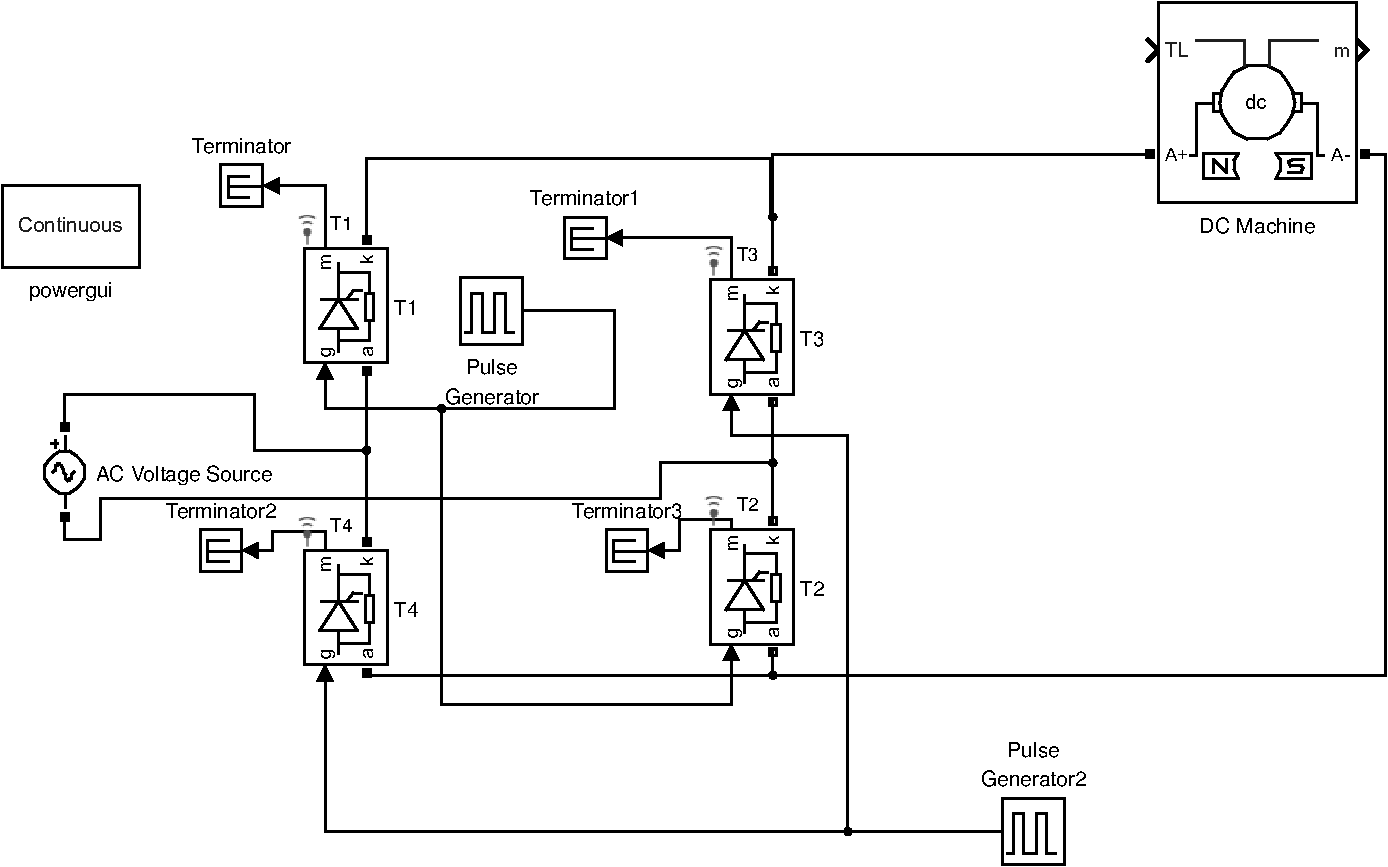
\includegraphics[width=\linewidth]{matlab/sim3}
	\caption{Acionamento de motor DC através de retificador monofásico controlado}
	\label{fig:sim3}
\end{figure}

Simulamos a resposta do motor para ângulos de disparo de $0^\circ$ (figura \ref{fig:res4}) e $90^\circ$ (figura \ref{fig:res5}).

\begin{figure}[H]
	\centering
	\begin{subfigure}[b]{0.49\linewidth}
		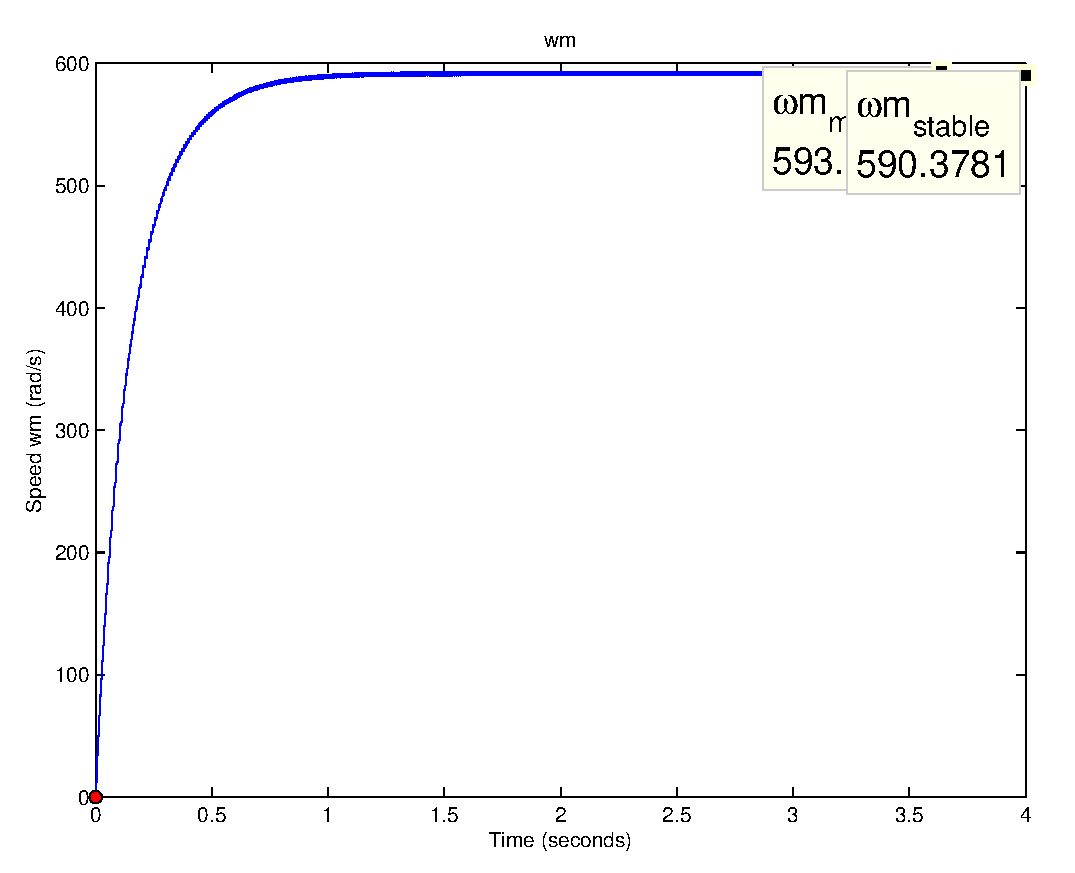
\includegraphics[width=\linewidth]{matlab/wm4}
		\caption{Velocidade Angular}
	\end{subfigure}
	\begin{subfigure}[b]{0.49\linewidth}
		\centering
		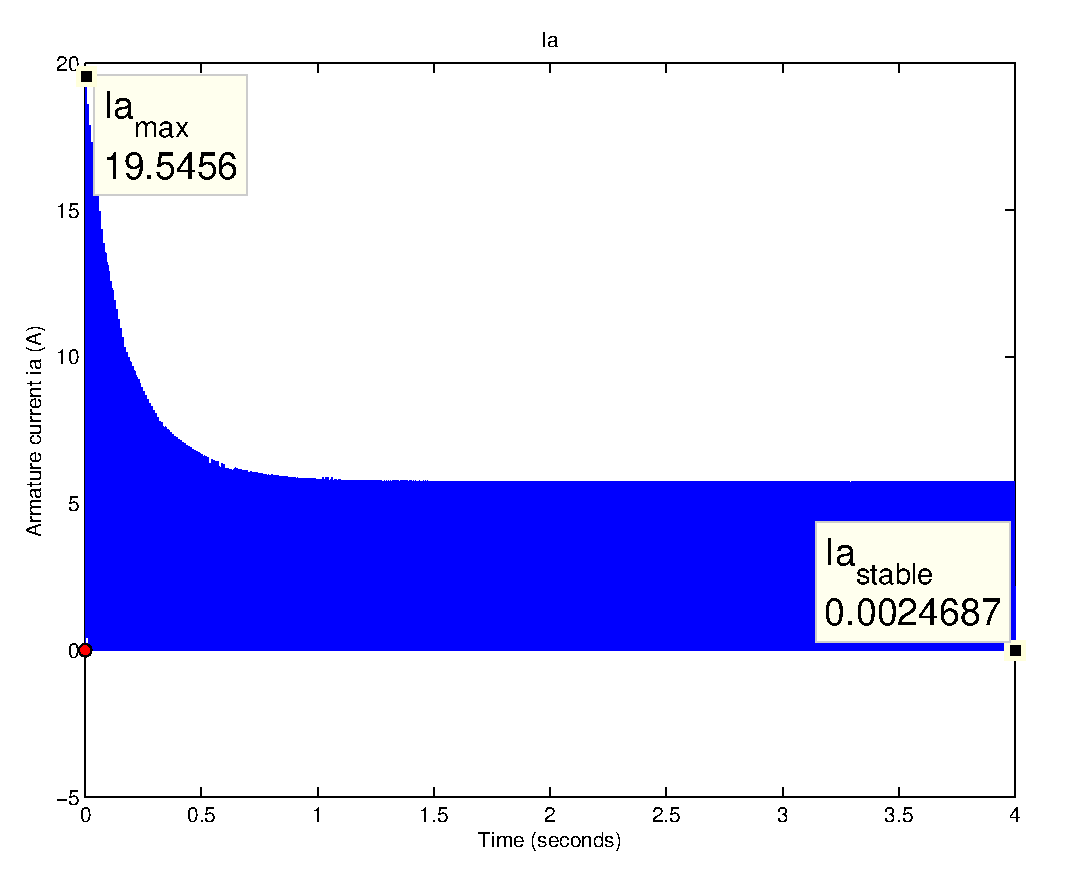
\includegraphics[width=\linewidth]{matlab/ia4}
		\caption{Corrente de armadura}
	\end{subfigure}
	\begin{subfigure}[b]{0.49\linewidth}
		\centering
		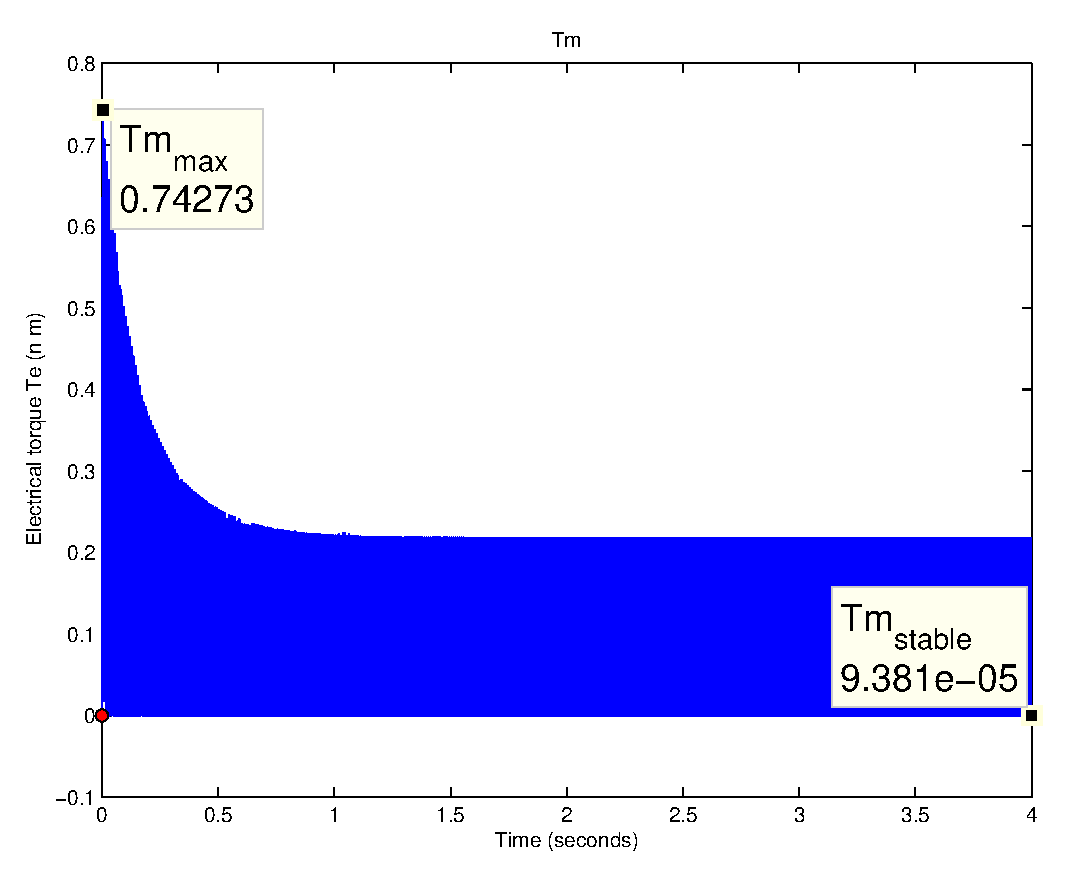
\includegraphics[width=\linewidth]{matlab/tm4}
		\caption{Torque do motor}
	\end{subfigure}
	\caption{Curvas de resposta do motor ângulo de disparo $0^\circ$}
	\label{fig:res4}
\end{figure}

\begin{figure}[H]
	\centering
	\begin{subfigure}[b]{0.49\linewidth}
		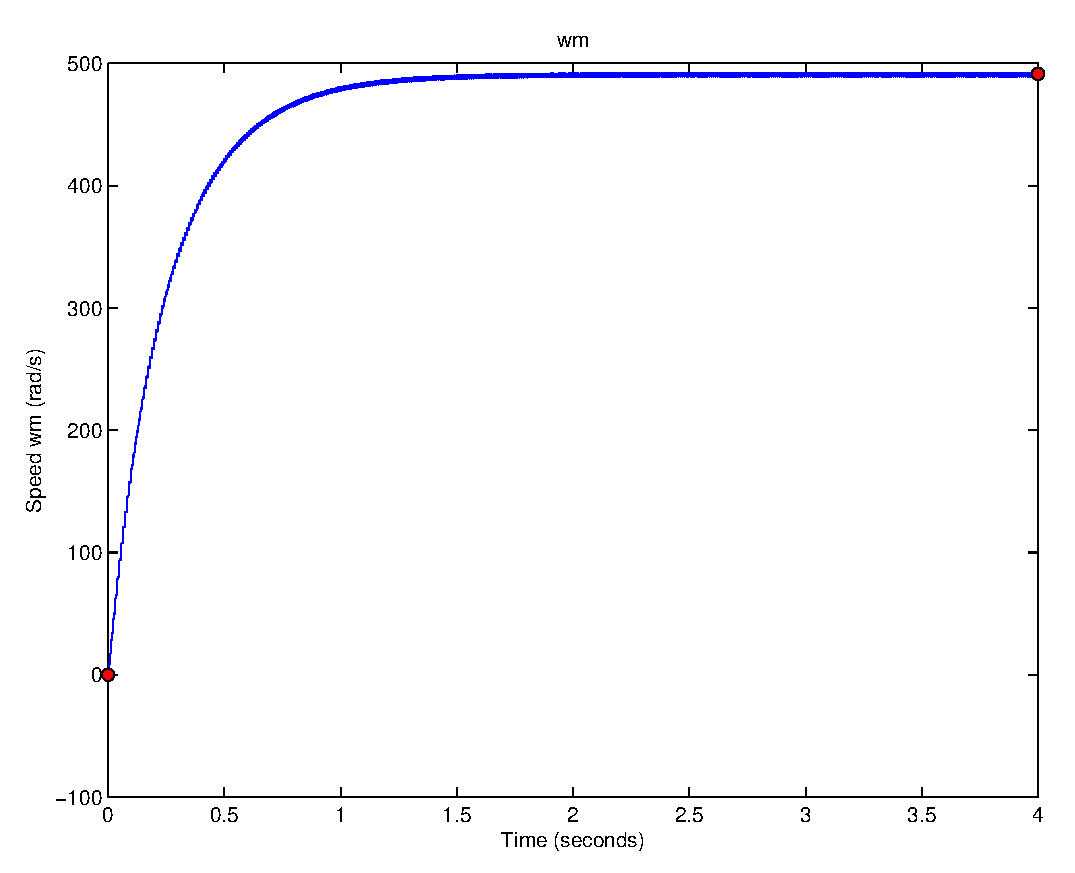
\includegraphics[width=\linewidth]{matlab/wm5}
		\caption{Velocidade Angular}
	\end{subfigure}
	\begin{subfigure}[b]{0.49\linewidth}
		\centering
		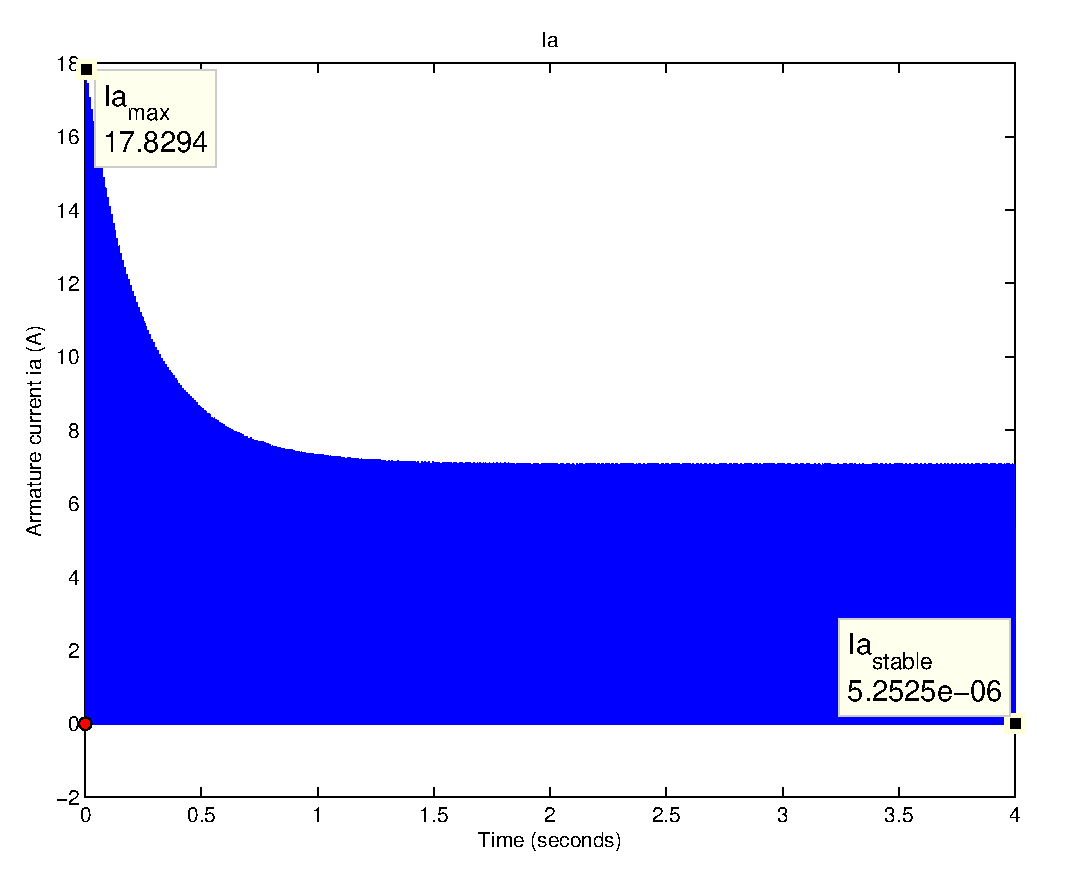
\includegraphics[width=\linewidth]{matlab/ia5}
		\caption{Corrente de armadura}
	\end{subfigure}
	\begin{subfigure}[b]{0.49\linewidth}
		\centering
		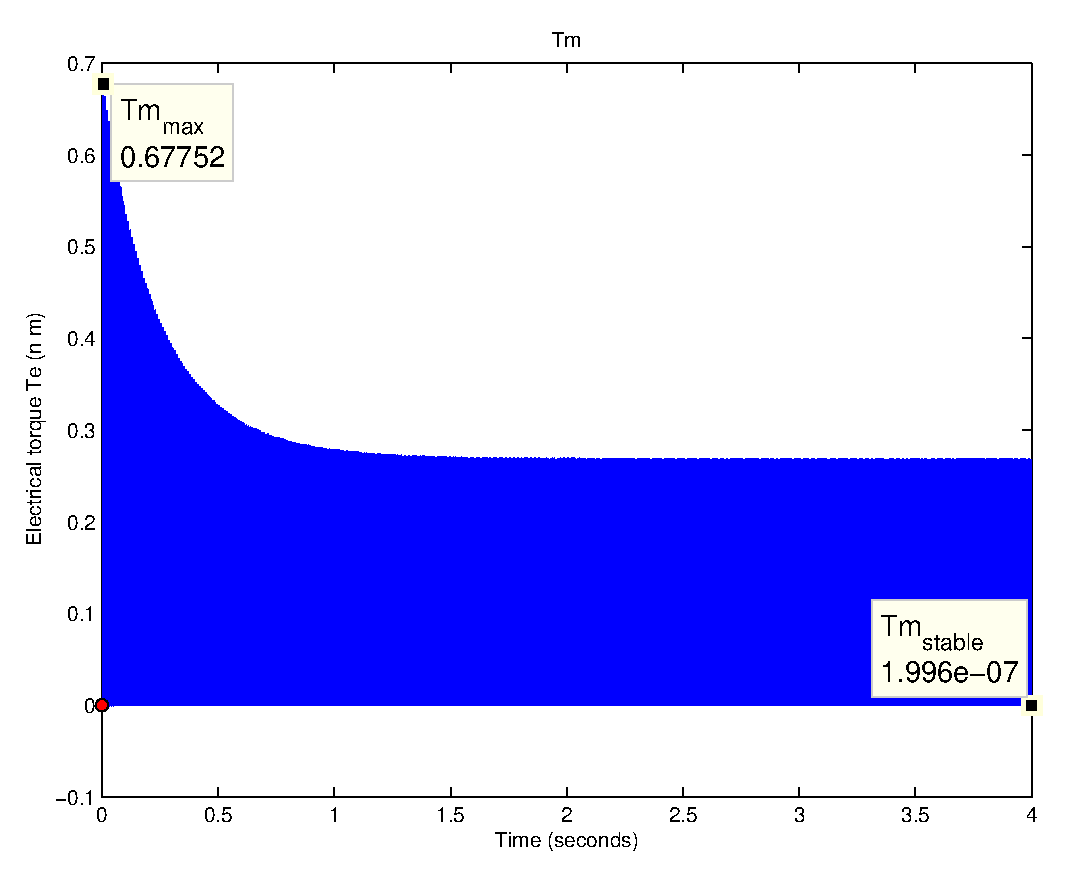
\includegraphics[width=\linewidth]{matlab/tm5}
		\caption{Torque do motor}
	\end{subfigure}
	\caption{Curvas de resposta do motor ângulo de disparo $90^\circ$}
	\label{fig:res5}
\end{figure}
Como podemos ver a oscilação de tensão gerada pelo retificador não pode ser sentida na velocidade do motor, porém ela afeta fortemente a corrente de armadura e o torque de saída. Também notamos que o efeito da mudança do ângulo de disparo é muito pequeno, mudando somente o tempo de resposta do circuito. Acreditamos que isso ocorre pois o motor encontra-se já saturado em ambas as configurações. Mudamos a fonte de 24 V rms para tensão de pico 24 V e rodamos as simulações novamente, obtendo as curvas de velocidade apresentadas na figura \ref{fig:res9}

\begin{figure}[H]
	\centering
	\begin{subfigure}[b]{0.49\linewidth}
		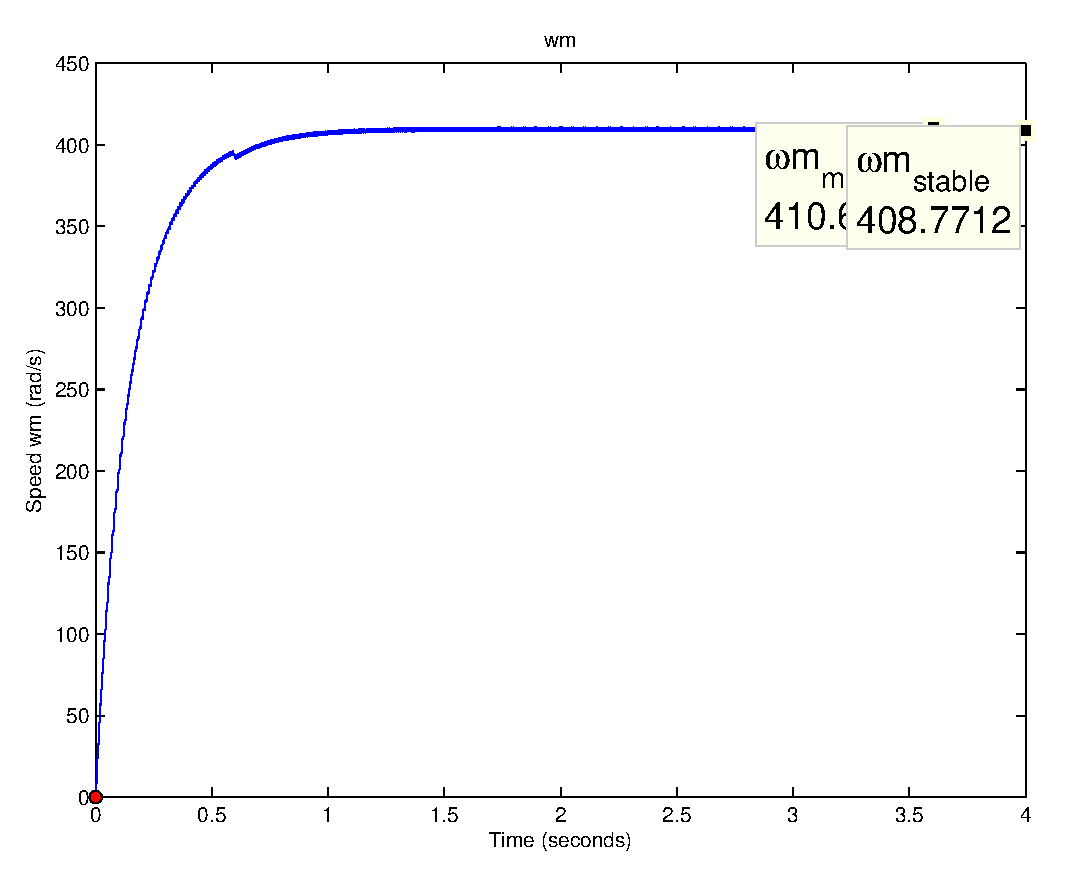
\includegraphics[width=\linewidth]{matlab/wm9}
		\caption{$0^\circ$}
	\end{subfigure}
	\begin{subfigure}[b]{0.49\linewidth}
		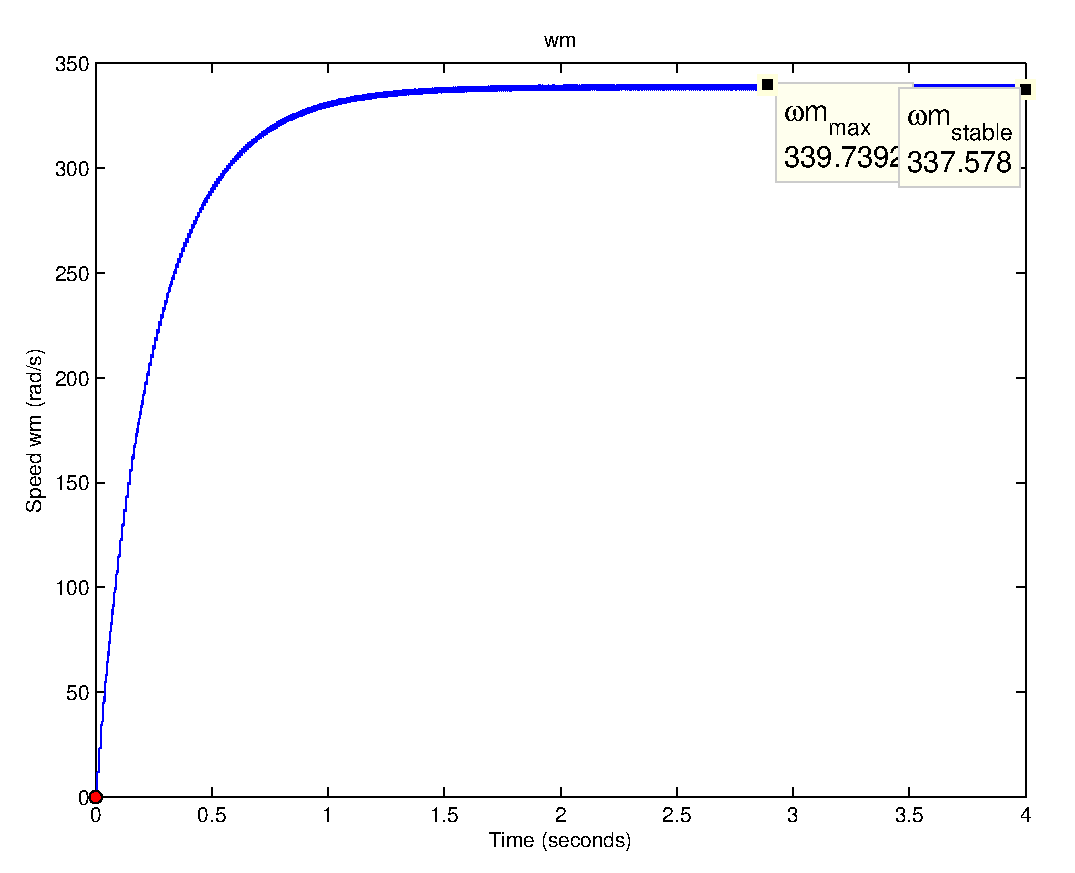
\includegraphics[width=\linewidth]{matlab/wm10}
		\caption{$90^\circ$}
	\end{subfigure}
	\caption{Velocidade do motor para diferentes ângulos de disparo}
	\label{fig:res9}
\end{figure}

Como podemos ver, agora o ângulo de disparo tem uma influência considerável na velocidade atingida pelo motor, conforme o esperado uma vez que ao alterar esse ângulo estamos alterando a tensão de armadura média aplicada.

Para resolver o problema das oscilações na corrente de armadura e no torque, conectamos um filtro capacitivo em nosso sistema (através de um capacitor de $0.5 F$ conectado em paralelo ao motor), conforme apresentado na figura \ref{fig:sim4} 

\begin{figure}[H]
	\centering
	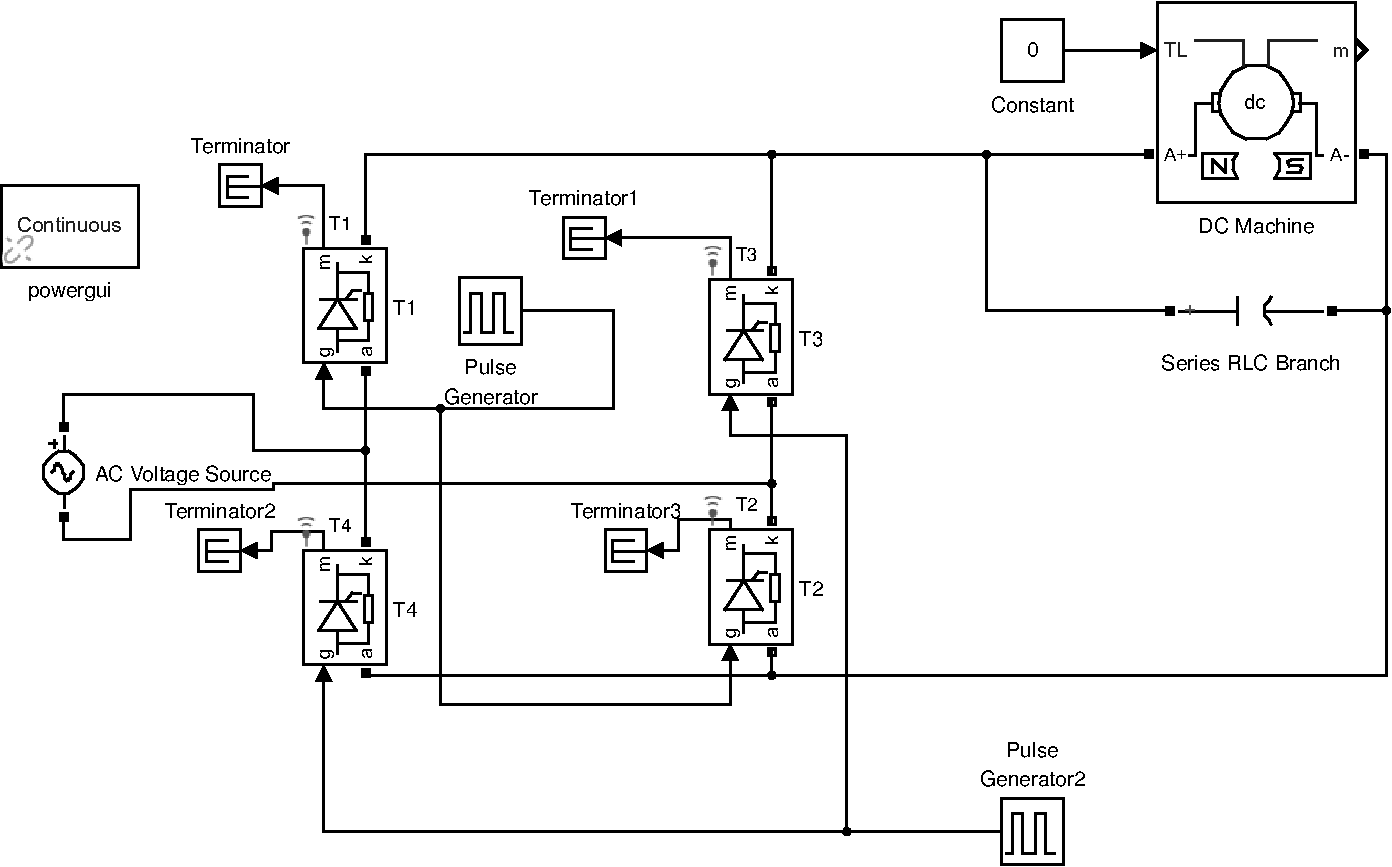
\includegraphics[width=\linewidth]{matlab/sim4}
	\caption{Acionamento de motor DC através de retificador monofásico controlado com filtro capacitivo}
	\label{fig:sim4}
\end{figure}

Rodamos novamente as simulações para ângulos de disparo de (figura \ref{fig:res6}) e $90^\circ$ (figura \ref{fig:res7}) (com tensão 24 V rms).

\begin{figure}[H]
	\centering
	\begin{subfigure}[b]{0.49\linewidth}
		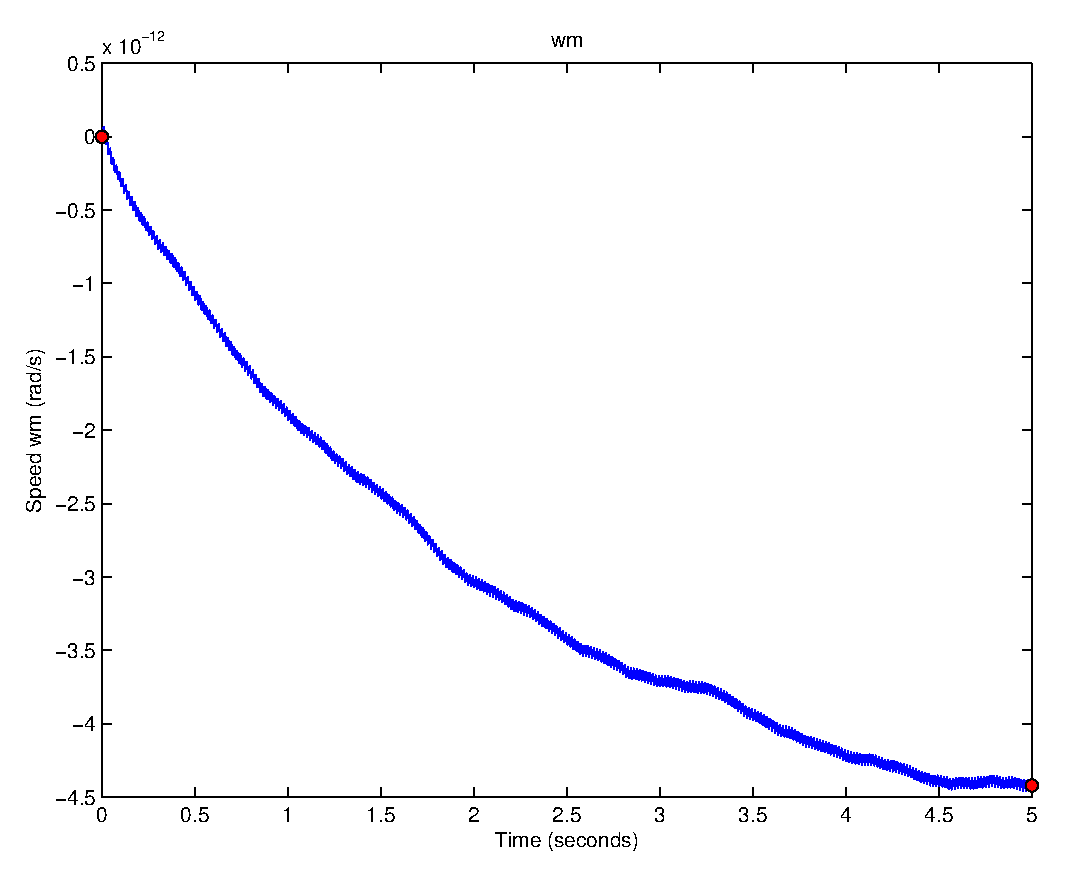
\includegraphics[width=\linewidth]{matlab/wm6}
		\caption{Velocidade Angular}
	\end{subfigure}
	\begin{subfigure}[b]{0.49\linewidth}
		\centering
		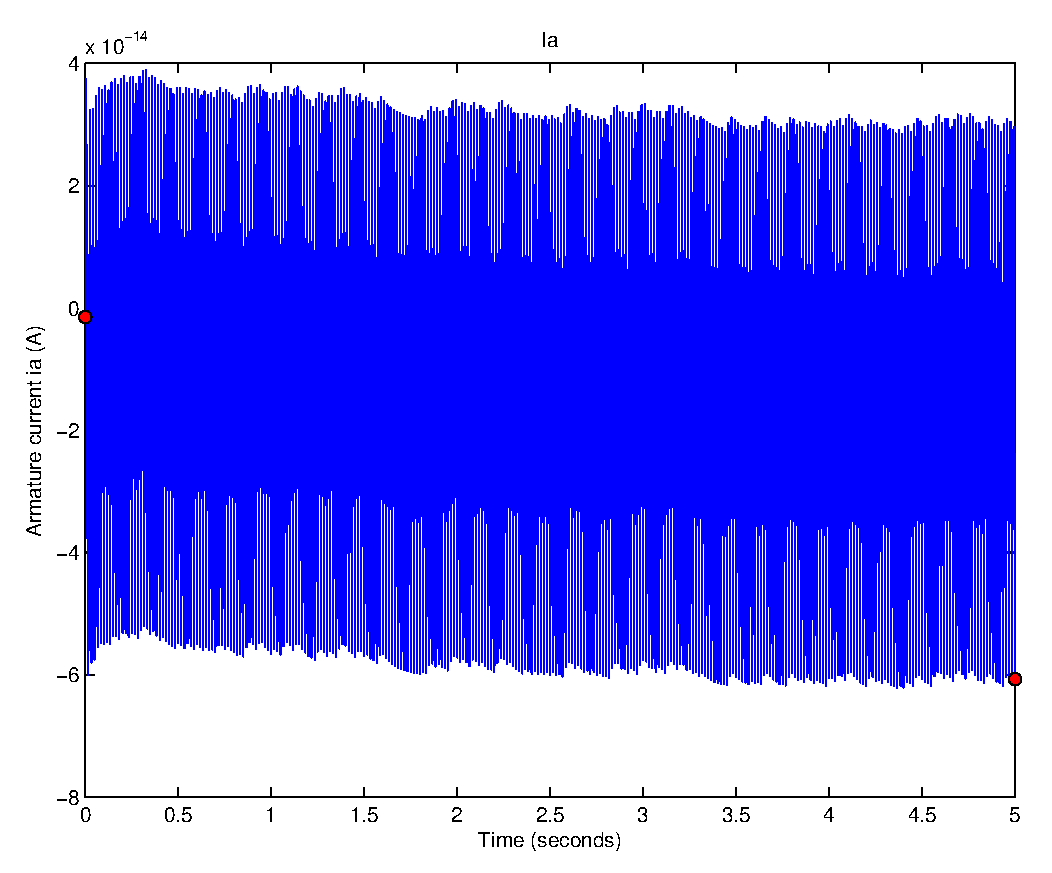
\includegraphics[width=\linewidth]{matlab/ia6}
		\caption{Corrente de armadura}
	\end{subfigure}
	\begin{subfigure}[b]{0.49\linewidth}
		\centering
		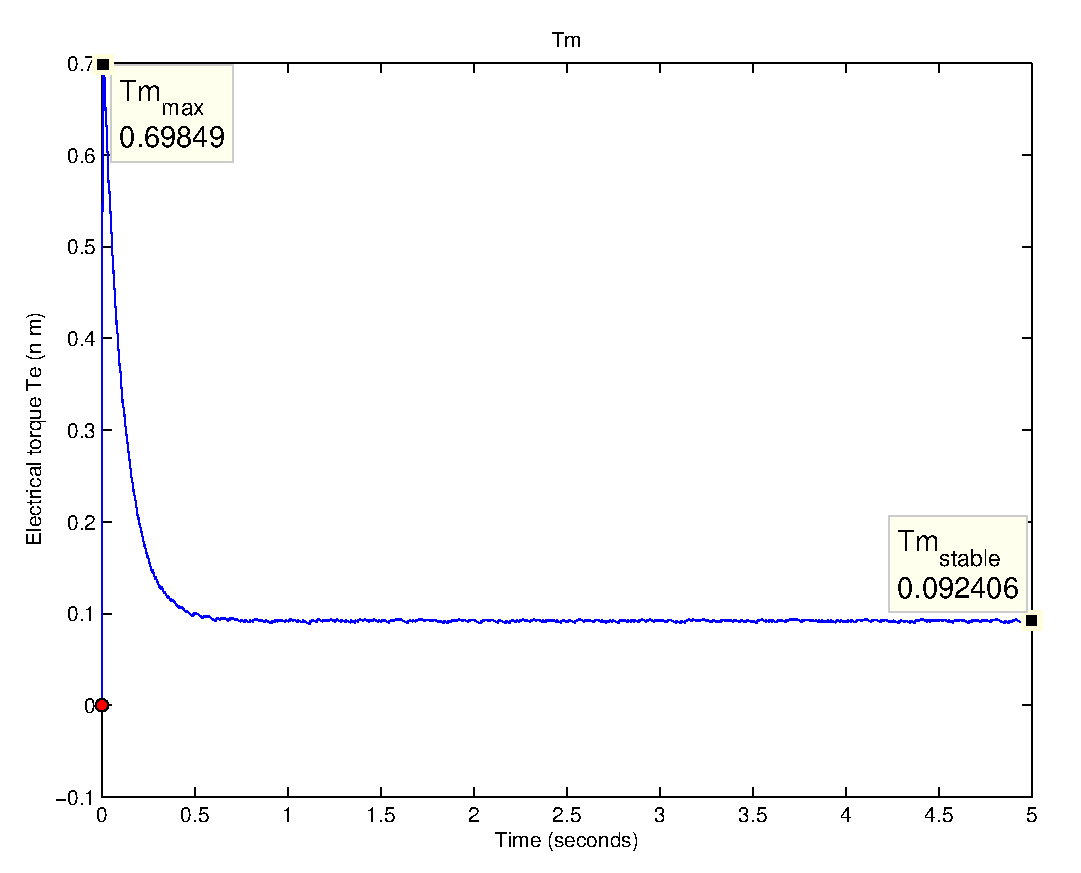
\includegraphics[width=\linewidth]{matlab/tm6}
		\caption{Torque do motor}
	\end{subfigure}
	\caption{Curvas de resposta do motor ângulo de disparo $0^\circ$}
	\label{fig:res6}
\end{figure}

\begin{figure}[H]
	\centering
	\begin{subfigure}[b]{0.49\linewidth}
		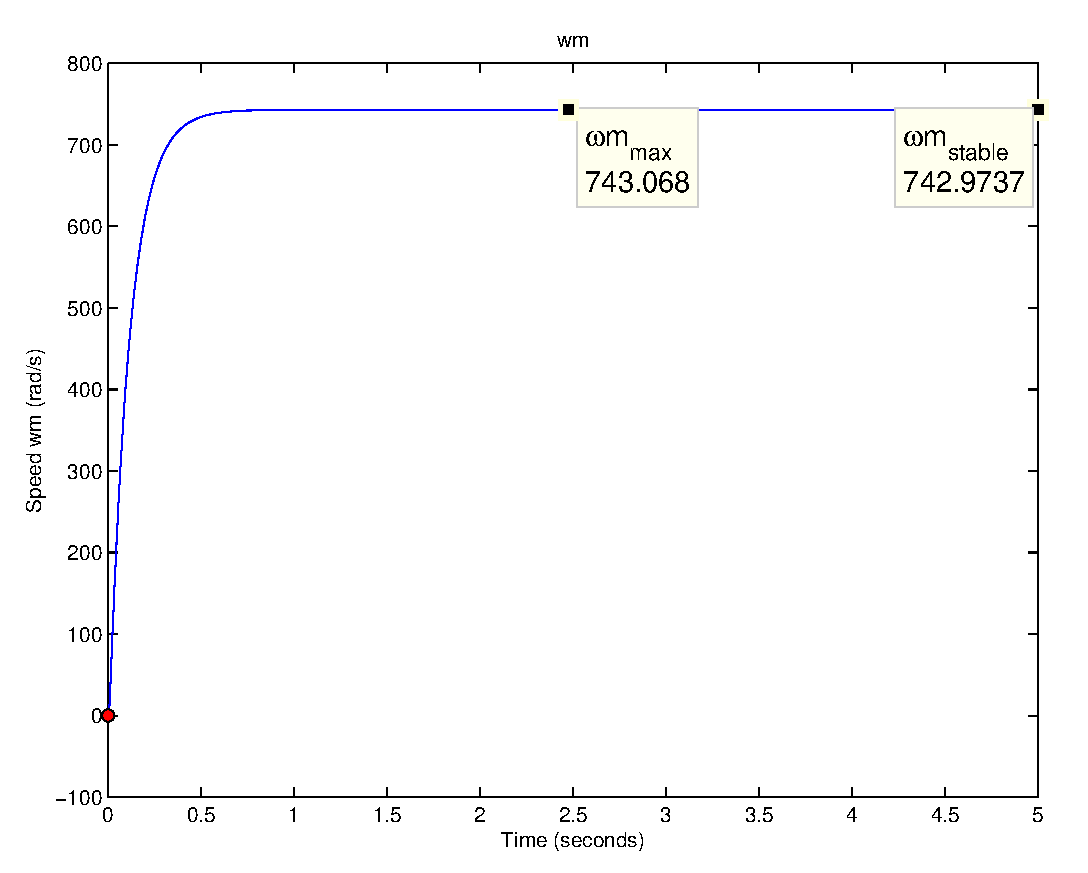
\includegraphics[width=\linewidth]{matlab/wm7}
		\caption{Velocidade Angular}
	\end{subfigure}
	\begin{subfigure}[b]{0.49\linewidth}
		\centering
		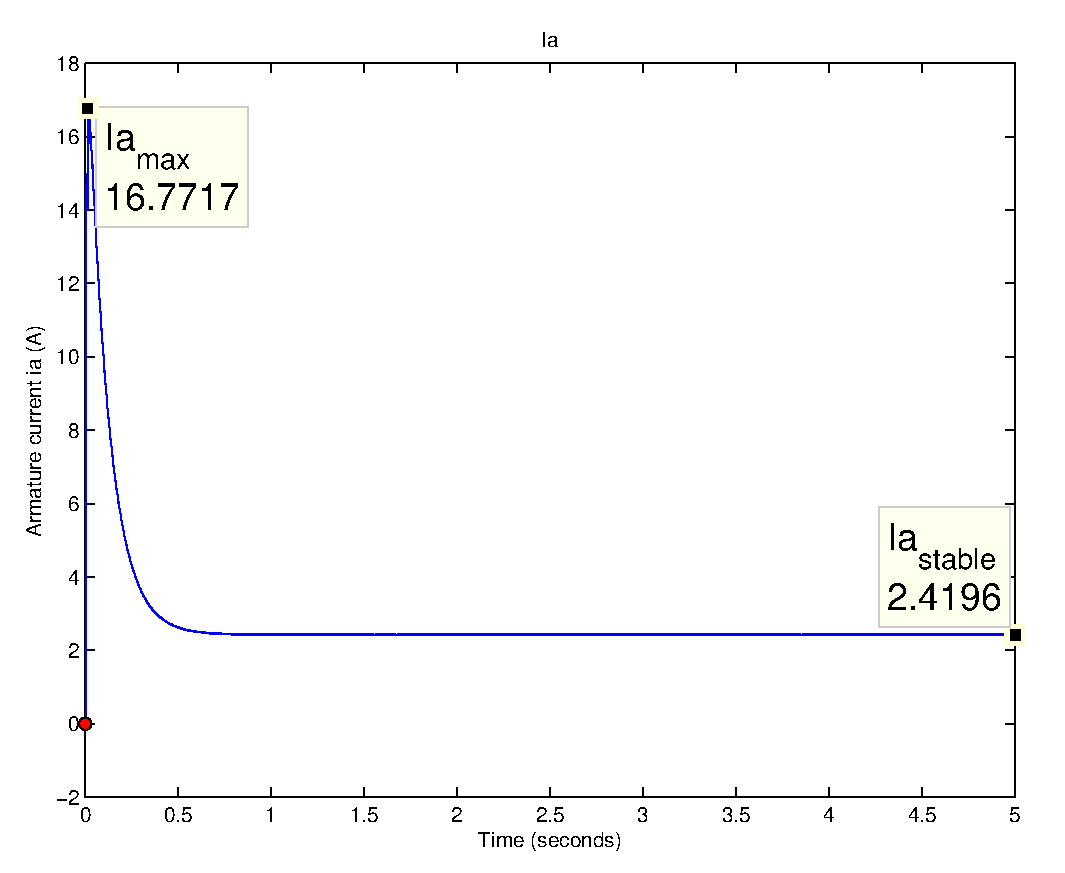
\includegraphics[width=\linewidth]{matlab/ia7}
		\caption{Corrente de armadura}
	\end{subfigure}
	\begin{subfigure}[b]{0.49\linewidth}
		\centering
		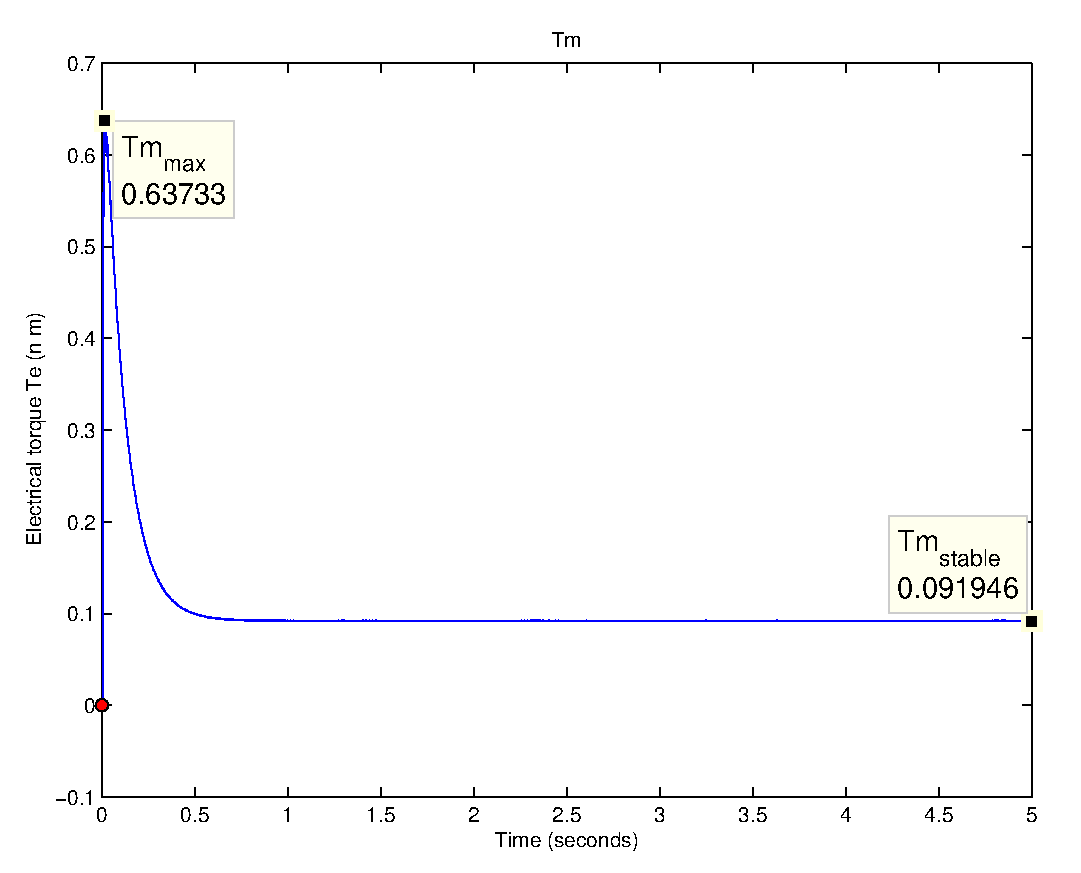
\includegraphics[width=\linewidth]{matlab/tm7}
		\caption{Torque do motor}
	\end{subfigure}
	\caption{Curvas de resposta do motor ângulo de disparo $90^\circ$}
	\label{fig:res7}
\end{figure}
Podemos ver que o filtro conseguiu cortar efetivamente as oscilações na corrente e no torque. Devemos lembrar que o motor é uma carga do tipo RLE, logo a tensão de saída do retificador só assume valores maiores que a tensão gerada pelo motor (E) quando a tensão da fonte é maior que E em valor absoluto. Como essa janela é muito pequena o ângulo de disparo tem pouco efeito no funcionamento do motor uma vez que sua velocidade está alta o suficiente.

\subsection{Acionamento de motor DC com conversor dual}
Colocamos um circuito de acionamento com conversor dual alimentado por uma fonte alternada (24 V rms@60 Hz) e com um capacitor de 1 F em paralelo, conforme pode ser visto nas figuras \ref{fig:sim5} e \ref{fig:sim6}.
\begin{figure}[H]
	\centering
	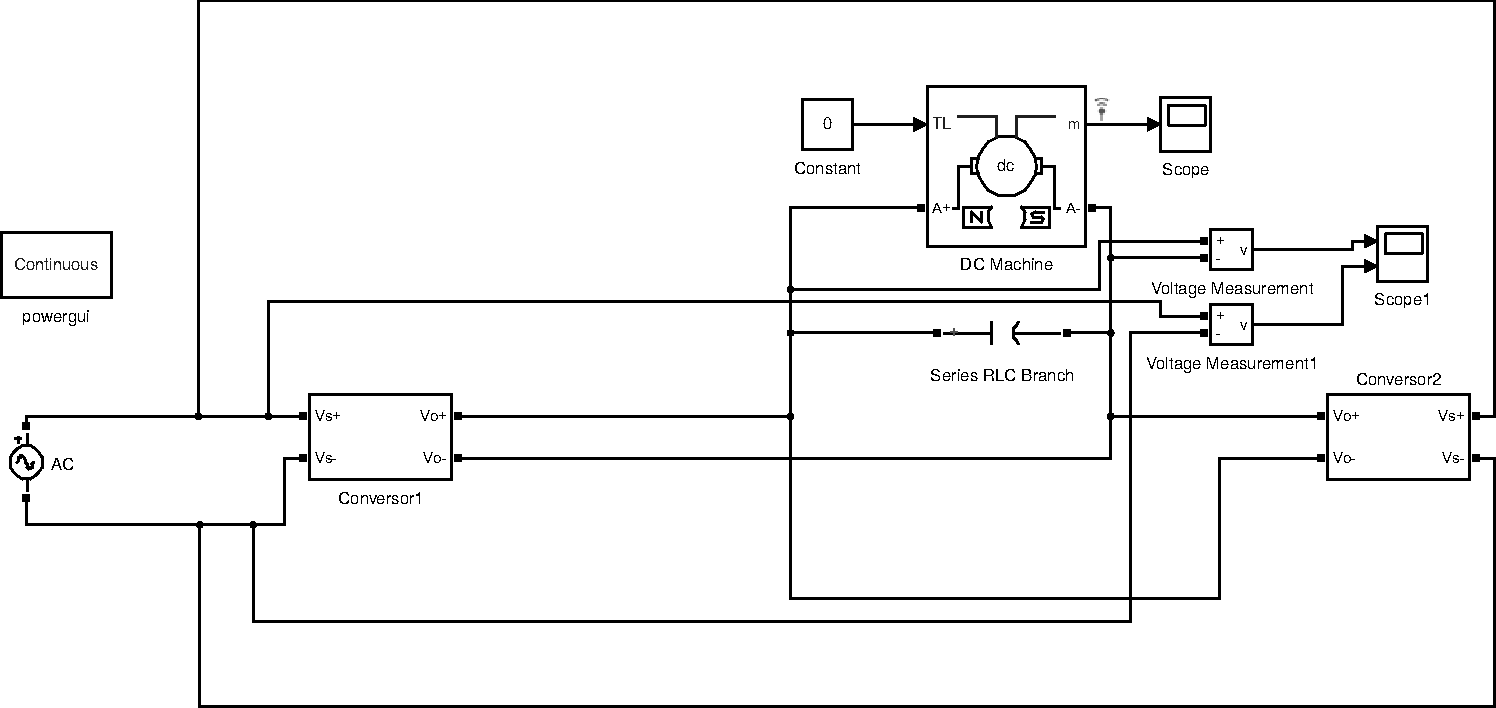
\includegraphics[width=\linewidth]{matlab/sim5}
	\caption{Acionamento de motor DC através de conversor dual}
	\label{fig:sim5}
\end{figure}
\begin{figure}[H]
	\centering
	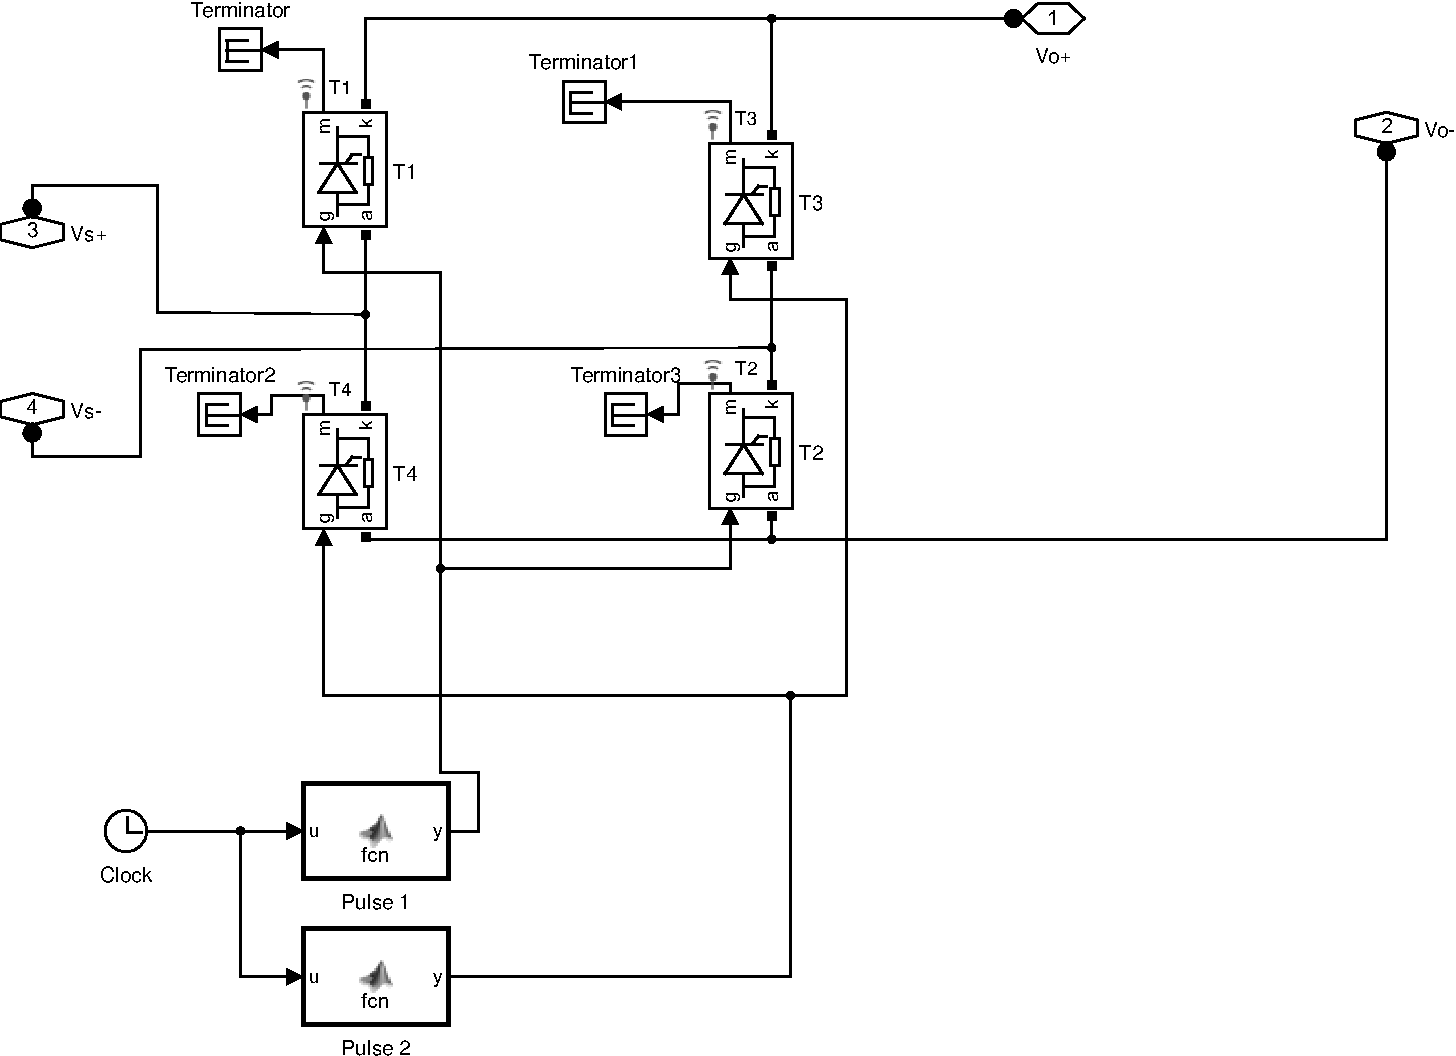
\includegraphics[width=\linewidth]{matlab/sim6}
	\caption{Detalhes do submódulo conversor}
	\label{fig:sim6}
\end{figure}

Simulamos um ciclo completo de operação do motor variando a velocidade de rotação entre os valores máximos direto e reverso segundo o ciclo $\omega = [0,\omega_+,\omega_-, 0]$. Para isso controlamos o ângulo de disparo dos conversores (ativando eles no máximo com o ângulo de disparo $\alpha = 0^\circ$ e desativando com $\alpha = 180^\circ$). Para colocar o motor em rotação máxima positiva ativamos o conversor um com ângulo de disparo $\alpha_1 = 0^\circ$ e o conversor dois com $\alpha_2 = 180^\circ$. Para rotação máxima reversa $\alpha_1 = 180^\circ$ e $\alpha_2 = 0^\circ$ e para $\alpha_1 = 90^\circ$ e $\alpha_2 = 90^\circ$. Os resultados da simulação estão apresentados na figura \ref{fig:res8}.
\begin{figure}[H]
	\centering
	\begin{subfigure}[b]{0.49\linewidth}
		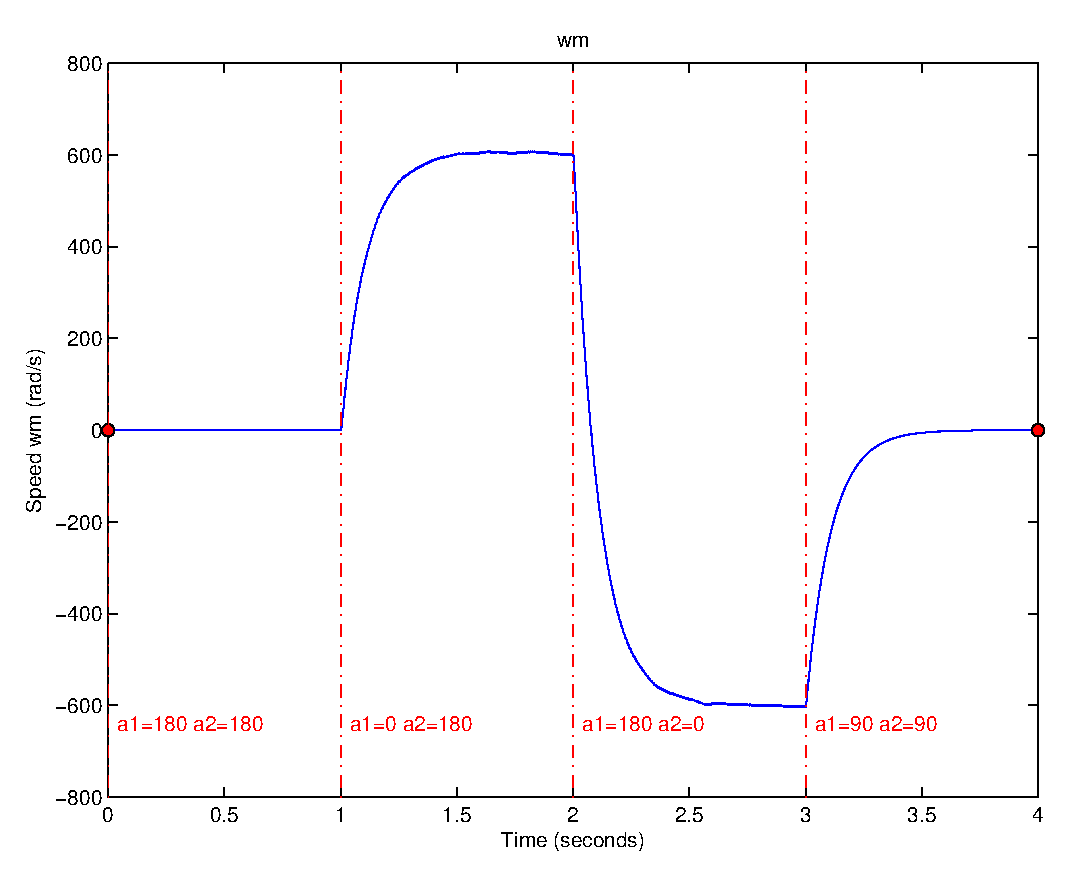
\includegraphics[width=\linewidth]{matlab/wm8}
		\caption{Velocidade Angular}
	\end{subfigure}
	\begin{subfigure}[b]{0.49\linewidth}
		\centering
		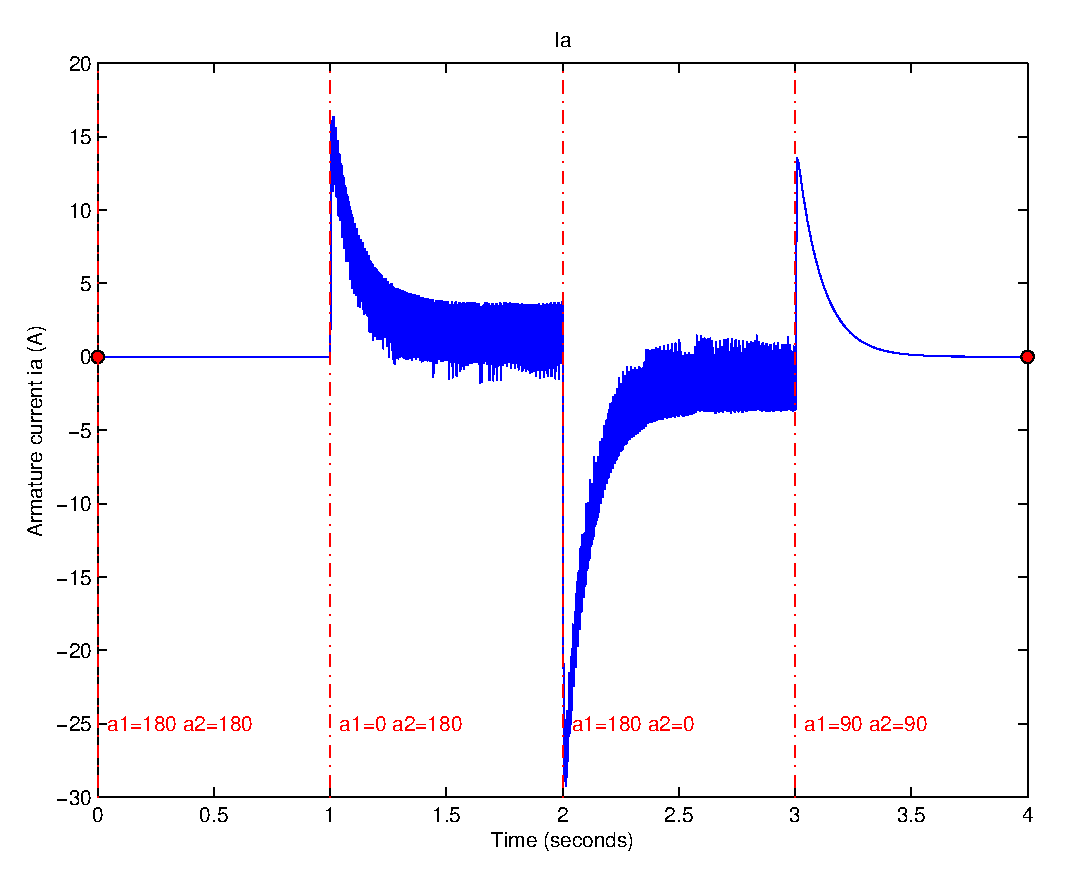
\includegraphics[width=\linewidth]{matlab/ia8}
		\caption{Corrente de armadura}
	\end{subfigure}
	\begin{subfigure}[b]{0.49\linewidth}
		\centering
		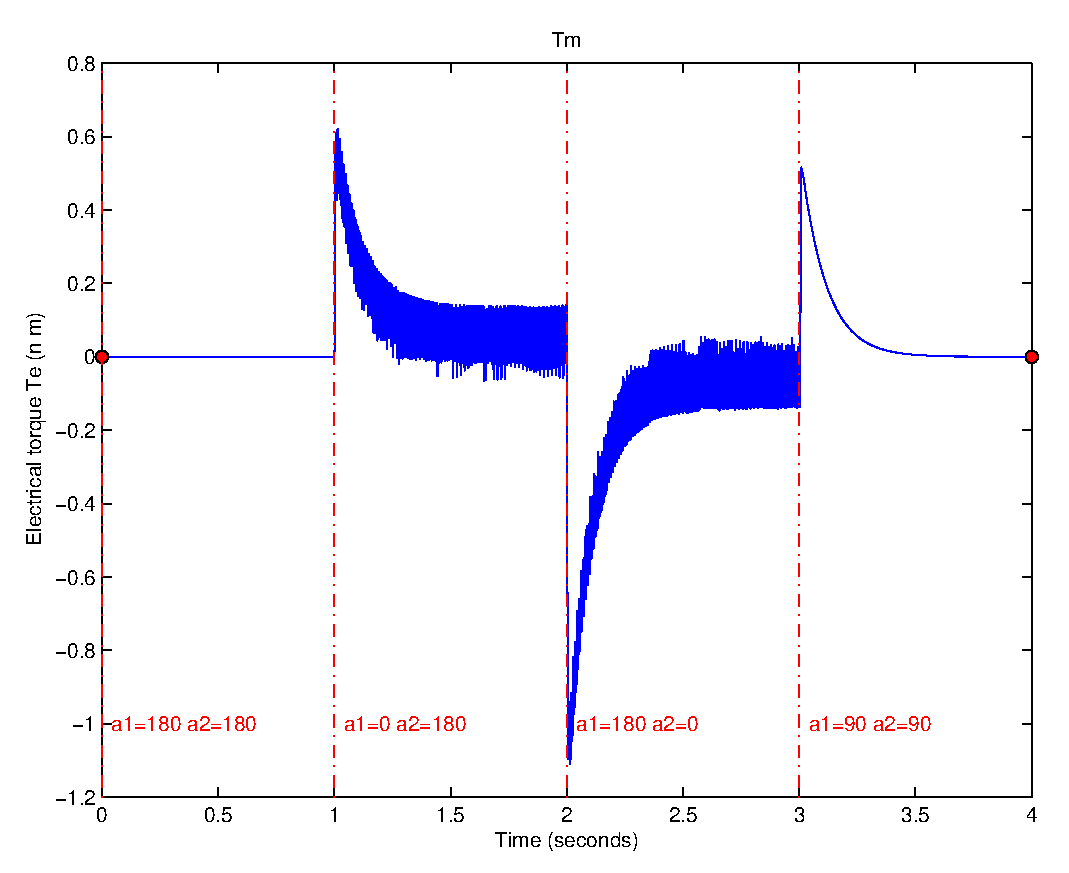
\includegraphics[width=\linewidth]{matlab/tm8}
		\caption{Torque do motor}
	\end{subfigure}
	\caption{Ciclo completo do motor acionado por conversor dual}
	\label{fig:res8}
\end{figure}
%TODO Comentar algo tipo pq diabos tem tanto ruido
\section{Questões}
\subsection{Princípio de funcionamento de um motor DC}
%TODO
\subsection{Quadrantes dos conversores}
%TODO
\subsection{Controle em malha aberta}
%TODO
\bibliography{mybib}
\end{document}

